\documentclass[12pt,a4j,oneside,titlepage,fleqn]{jsbook}
%
%% パッケージ
\usepackage[dvipdfmx]{hyperref}
\usepackage{pxjahyper}
\usepackage{geometry}
\usepackage{amsmath}
\usepackage{amssymb}
\usepackage{txfonts}
\usepackage{bm}
\usepackage{titlesec}
\usepackage[dvipdfmx]{graphicx}
\usepackage{booktabs}
%
%% 設定
\geometry{top=20truemm,bottom=15truemm,left=25truemm,right=10truemm}
\setlength{\fullwidth}{175truemm}
\linespread{0.97}  % 1 ページ 40 行
\pagestyle{plain}
\setcounter{secnumdepth}{3}
\setcounter{tocdepth}{3}
\renewcommand{\prechaptername}{}
\renewcommand{\postchaptername}{.}
\renewcommand{\thesection}{\thechapter$\cdot$\arabic{section}}
\renewcommand{\thesubsection}{\thesection$\cdot$\arabic{subsection}}
\renewcommand{\thesubsubsection}{\thesubsection$\cdot$\arabic{subsubsection}}
\titleformat{\chapter}{\centering\sffamily\gtfamily\Large}{\prechaptername\thechapter\postchaptername}{1zw}{}
\titleformat{\section}{\sffamily\gtfamily\large}{\thesection}{1zw}{}
\titleformat{\subsection}{\sffamily\gtfamily\normalsize}{\thesubsection}{1zw}{}
\titleformat{\subsubsection}{\sffamily\gtfamily\normalsize}{\thesubsubsection}{1zw}{}
\titlespacing{\chapter}{0pt}{0pt}{\baselineskip}
\titlespacing{\section}{1zw}{\baselineskip}{0pt}
\titlespacing{\subsection}{1zw}{\baselineskip}{0pt}
\titlespacing{\subsubsection}{1zw}{\baselineskip}{0pt}
\renewcommand{\figurename}{Fig.~}
\renewcommand{\tablename}{Table~}
\setlength{\mathindent}{2em}
\setlength{\jot}{\baselineskip}
%
%% 表紙
\renewcommand{\maketitle}{
\begin{titlepage}
 \setcounter{page}{0}
 \begin{center}
  \vspace*{8\baselineskip}
  {○○○○年度卒業論文} \\[2\baselineskip]
  {\Large へたれテンプレート} \\[9\baselineskip]
  {○○○○年○月} \\[2\baselineskip]
  {東京理科大学理工学部機械工学科} \\[\baselineskip]
  {○○研究室} \\[3\baselineskip]
  {75*****  機械 工作}
 \end{center}
\end{titlepage}
}
%
%%%%%%%%%%%%%%%%%%%%%%%%%%%%%%%%%%%%%%%%
%
\begin{document}
%
%% 設定
\setlength{\abovedisplayskip}{\baselineskip}
\setlength{\belowdisplayskip}{\baselineskip}
%
%% 前付け
\frontmatter
\maketitle
\tableofcontents
%
%% 本文
\mainmatter
\chapter{緒言}
\section{へたれテンプレートとは?}
へたれテンプレートとは,初心者が熟練者に成長する過程でぐちゃぐちゃに改変される土台となるテンプレートです.
へたれテンプレートがどれだけぐちゃぐちゃに改変されたかを見ると,あなたがどれだけ \LaTeX に習熟したかがわかります.

\chapter{基本的な使い方}
\section{PDF ファイル作成方法}
このへたれテンプレートには Makefile が付属するので
\begin{verbatim}
% make
\end{verbatim}
で PDF ファイルを作成できます.
\section{コメントアウト}
\% 以降はコメントアウトされます.
% 以降はコメントアウトされます.
\section{段落}
空行を入れると改段落されます.
空行を入れると改段落されます.
空行を入れると改段落されます.
空行を入れると改段落されます.
空行を入れると改段落されます.
空行を入れると改段落されます.
空行を入れると改段落されます.

改段落したくない場所には空行を入れないようにしましょう.
改段落したくない場所には空行を入れないようにしましょう.
% コメント行は改段落されません.
改段落したくない場所には空行を入れないようにしましょう.
%
改段落したくない場所には空行を入れないようにしましょう.
改段落したくない場所には空行を入れないようにしましょう.
\section{箇条書き}
箇条書きです.
\begin{itemize}
 \item 有限要素法
 \item 有限差分法
 \item 有限体積法
\end{itemize}

番号の箇条書きです.
\begin{enumerate}
 \item 有限要素法
 \item 有限差分法
 \item 有限体積法
\end{enumerate}
\section{図と表}
図~\ref{fig:okadakenkun} に図を示します.
表~\ref{tab:parameters} に表を示します.
図表はページの上部や下部の適当な位置に自動的に配置されます.
label コマンドと ref コマンドを用いることで図表番号が自動的に対応します.
\begin{figure}[tbp]
 \centering
 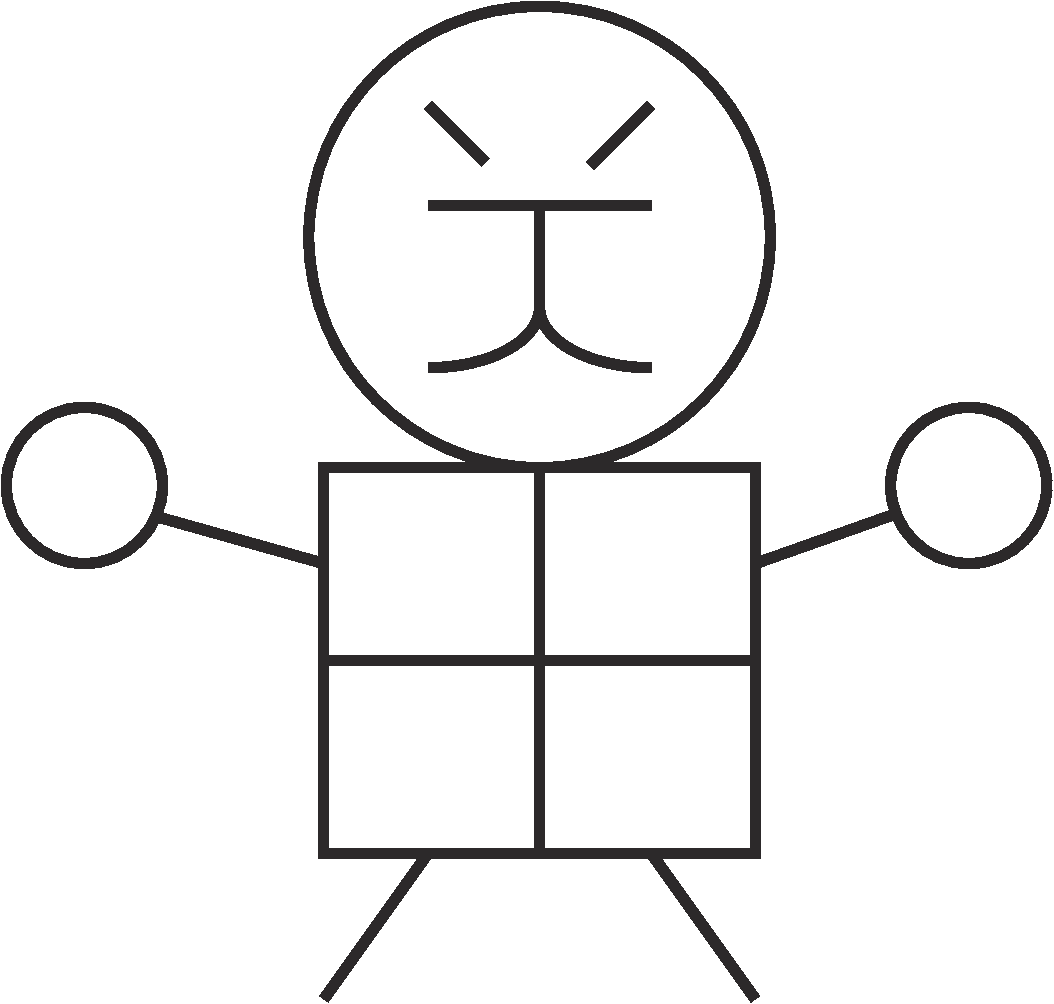
\includegraphics[width=0.3\hsize]{fig/okadakenkun.pdf}  % eps,png,jpg なども可
 \caption{Okadaken-kun. He is a mascot of Okada Lab.}\label{fig:okadakenkun}
\end{figure}
\begin{table}[tbp]
 \centering
 \caption{Young's modulus and Poisson's ratio.}\label{tab:parameters}
 \begin{tabular}{rl}
  \toprule
  Young's modulus (GPa) & 210 \\
  Poisson's ratio & 0.3 \\
  \bottomrule
 \end{tabular}
\end{table}
\section{数式}
数式は
\begin{equation}
 \bm{f} = -k \bm{u}
\end{equation}
のように記します.
複数の数式は
\begin{align}
 \bm{f}_1 = -k \bm{u}_1 \\
 \bm{f}_2 = -k \bm{u}_2
\end{align}
のように記します.
本文中の数式は $\bm{f}$ や $\bm{f} = -k \bm{u}$ のように記します.

label コマンドを付けて
\begin{equation}
 \bm{f} = m \frac{d^2 \bm{u}}{d t^2}\label{eq:motion}
\end{equation}
のように記すと,ref コマンドで式 (\ref{eq:motion}) のように参照できます.
\section{文献の引用}
○○の研究(Okada et al., 1988)のように引用します.
Okada et al.\ (1988) は○○を研究したという書き方の引用もできます.
日本語の場合は,○○の研究(岡田他, 1998)のように引用します.
岡田他(1998)は○○を研究したという書き方の引用もできます.

% \chapter{重合パッチ法}
\section{重合パッチ法の理論}
重合パッチ法による解析では,
全体の構造をIGAグローバルパッチで離散化し,
詳細な領域ではIGAローカルパッチで離散化し,
グローバルパッチとローカルパッチを重ね合わせて解析を行う.
図~\ref{fig:Concept S-IGA}に示すように,グローバル領域$\Omega^G$,ローカル領域$\Omega^L$,グローバル領域の境界$\Gamma^G$,
ローカル領域の境界$\Gamma^L$,グローバル領域上のローカル領域の境界$\Gamma^{GL}$とする.

\begin{figure}[htbp]
  \centering
  \includegraphics[keepaspectratio, scale = 0.7]
  {fig/重合パッチ_v2.ai}
  \caption{Concept of S-IGA}
  \label{fig:Concept S-IGA}
\end{figure}

\noindent
添え字$G,L$はそれぞれグローバル領域$\Omega^G$,ローカル領域$\Omega^L$に関する物理量量であることを示す表記である.
$\Omega^G,\Omega^L$ではそれぞれ独立の変位場$\boldsymbol{u}^G,\boldsymbol{u}^L$が定義されており,$\Omega^L$上での実際の変位は
$\Omega^G,\Omega^L$での変位を重ね合わせた和で以下のように定義される.

\begin{equation}
  \label{eq:ugul}
  \boldsymbol{u} = \left \{
    \begin{array}{l}
      \boldsymbol{u}^G  \ \ \ \quad \qquad $in$ \quad \Omega^G \cap \overline{\Omega^L}\\
      \boldsymbol{u}^G+\boldsymbol{u}^L \ \ \ \quad $in$ \quad \Omega^L
    \end{array}
  \right.
\end{equation}

\noindent
また,$\Gamma^{GL}$での変位の$C^0$連続性を保証するため以下のような条件を課す.

\begin{equation}
  \boldsymbol{u}^L = \boldsymbol{0} \ \ \ \quad $on$ \quad \Gamma^{GL}
\end{equation}

\noindent
式~(\ref{eq:ugul})を偏微分することで,ひずみは以下のように表される.

\begin{equation}
  \boldsymbol{\varepsilon} = \left \{
    \begin{array}{l}
      \boldsymbol{L}\boldsymbol{u}^G = \boldsymbol{\varepsilon}^G \ \ \ \ \ \  \qquad \qquad \qquad \qquad \qquad \quad $in$ \quad \Omega^G \cap \overline{\Omega^L}\\
      \boldsymbol{L}(\boldsymbol{u}^G+\boldsymbol{u}^L)=\boldsymbol{L}\boldsymbol{u}^G+\boldsymbol{L}\boldsymbol{u}^L=\boldsymbol{\varepsilon}^G+\boldsymbol{\varepsilon}^L \qquad $in$ \quad \Omega^L
    \end{array}
  \right.
\end{equation}

\noindent
ここで,$\boldsymbol{L}$は,式~(\ref{eq:L})で表される二次元の微分作用素である.
領域$\Omega^G$,領域$\Omega^L$において,変位場及びひずみ場は形状関数を用いて離散化され,以下のように表される.

\begin{eqnarray}
  \boldsymbol{u}^G&=\boldsymbol{N}^G\boldsymbol{d}^G\\
  \boldsymbol{u}^L&=\boldsymbol{N}^L\boldsymbol{d}^L\\
  \boldsymbol{\varepsilon}^G&=\boldsymbol{B}^G\boldsymbol{u}^G\\
  \boldsymbol{\varepsilon}^L&=\boldsymbol{B}^L\boldsymbol{u}^L
\end{eqnarray}

\noindent
ここで,$\boldsymbol{N}^G$,$\boldsymbol{N}^L$はNURBS基底関数マトリクス,
$\boldsymbol{d}^G,\boldsymbol{d}^L$はコントロールポイント変位ベクトル,
$\boldsymbol{B}^G$,$\boldsymbol{B}^L$は変位ひずみマトリクスである.
このときグローバルパッチとローカルパッチの
コントロールポイントやノットベクトルが一致する必要はない.

上記の仮定を仮想仕事の原理に代入し,離散化されたつりあい方程式を導く.
ここで,仮想変位$\delta \boldsymbol{u}$,仮想ひずみ$\delta \boldsymbol{\varepsilon}$は,変位,ひずみと同様に
グローバルパッチとローカルパッチの重ね合わせで表現され,以下のように表される.

\begin{align}
  \delta \boldsymbol{u} &= \delta \boldsymbol{u}^G + \delta \boldsymbol{u}^L\\
  \delta \boldsymbol{\varepsilon} &= \delta \boldsymbol{\varepsilon}^G + \delta \boldsymbol{\varepsilon}^L
\end{align}

\noindent
線形弾性体の場合,仮想仕事の原理は以下のように表される.

\begin{equation}
  \label{eq:VW01}
  \int_\Omega \delta \boldsymbol{\varepsilon}^T \boldsymbol{D} \boldsymbol{\varepsilon} d\Omega
  = \int_\Omega \delta \boldsymbol{u}^T \boldsymbol{b} d\Omega + \int_{\Gamma^t} \delta \boldsymbol{u}^T \boldsymbol{t} d\Gamma
\end{equation}

\noindent
ここで,$\boldsymbol{D}$は弾性マトリクス,$\boldsymbol{b}$は体積力ベクトル,
$\boldsymbol{t}$は表面力ベクトルである.
式~(\ref{eq:VW01})の左辺を$\Omega^G\cap\overline{\Omega^L}$と$\Omega^L$の二つの領域に分割すると以下のように表される.

\begin{align}
  \int_{\Omega} \delta\boldsymbol{\varepsilon}^T\boldsymbol{D}\boldsymbol{\varepsilon} d\Omega
  &=\int_{\Omega^G\cap\overline{\Omega^L}} \delta{\boldsymbol{\varepsilon}^G}^T\boldsymbol{D}\boldsymbol{\varepsilon}^G d\Omega
  +\int_{\Omega^L} \delta({\boldsymbol{\varepsilon}^G}^T+{\boldsymbol{\varepsilon}^L}^T)\boldsymbol{D}(\boldsymbol{\varepsilon}^G+\boldsymbol{\varepsilon}^L) d\Omega \nonumber \\
  &=\int_{\Omega^G} \delta{\boldsymbol{\varepsilon}^G}^T\boldsymbol{D}\boldsymbol{\varepsilon}^G d\Omega
  +\int_{\Omega^L} \delta{\boldsymbol{\varepsilon}^G}^T\boldsymbol{D}\boldsymbol{\varepsilon}^L d\Omega
  +\int_{\Omega^L} \delta{\boldsymbol{\varepsilon}^L}^T\boldsymbol{D}\boldsymbol{\varepsilon}^G d\Omega
  +\int_{\Omega^L} \delta{\boldsymbol{\varepsilon}^L}^T\boldsymbol{D}\boldsymbol{\varepsilon}^L d\Omega
\end{align}

\noindent
式~(\ref{eq:VW01})の右辺についても同様に,$\Omega^G\cap\overline{\Omega^L}$と$\Omega^L$の二つの領域に分割すると以下のように表される.

\begin{equation}
  \int_\Omega \delta\boldsymbol{u}^T\boldsymbol{b} d\Omega+\int_{\Gamma^t} \delta\boldsymbol{u}^T\boldsymbol{t} d\Gamma
  =\int_{\Omega^G} \delta{\boldsymbol{u}^G}^T\boldsymbol{b} d\Omega+\int_{\Gamma^t} \delta{\boldsymbol{u}^G}^T\boldsymbol{t} d\Gamma
  +\int_{\Omega^L} \delta{\boldsymbol{u}^L}^T\boldsymbol{b} d\Omega+\int_{\Gamma^t} \delta{\boldsymbol{u}^L}^T\boldsymbol{t} d\Gamma
\end{equation}

\noindent
仮想変位の任意性から,離散化したつりあい方程式は以下のように表される.

\begin{equation}
  \label{eq:K_array}
  \begin{bmatrix}
    \boldsymbol{K}^G & \boldsymbol{K}^{GL} \\
    \boldsymbol{K}^{LG} & \boldsymbol{K}^L
  \end{bmatrix}
  \left\{
  \begin{array}{c}
    \boldsymbol{d}^G \\
    \boldsymbol{d}^L
  \end{array}
  \right\} =
  \left\{
  \begin{array}{c}
    \boldsymbol{f}^G \\
    \boldsymbol{f}^L
  \end{array}
  \right\}
\end{equation}

\noindent
ここで,以下のような式が成り立つ.

\begin{eqnarray}
  \boldsymbol{K}^G&=\int_{\Omega^G} {\boldsymbol{B}^G}^T\boldsymbol{D}\boldsymbol{B}^Gd\Omega\\
  \boldsymbol{K}^L&=\int_{\Omega^L} {\boldsymbol{B}^L}^T\boldsymbol{D}\boldsymbol{B}^Ld\Omega\\
  \boldsymbol{K}^{GL}&=\int_{\Omega^L} {\boldsymbol{B}^G}^T\boldsymbol{D}\boldsymbol{B}^Ld\Omega\\
  \boldsymbol{K}^{LG}&=\int_{\Omega^L} {\boldsymbol{B}^L}^T\boldsymbol{D}\boldsymbol{B}^Gd\Omega\\
  \boldsymbol{f}^{G}&=\int_{\Omega^G} {\boldsymbol{N}^G}^T\boldsymbol{b}d\Omega+\int_{\Gamma^t} {\boldsymbol{N}^G}^T\boldsymbol{t}d\Gamma\\
  \boldsymbol{f}^{L}&=\int_{\Omega^L} {\boldsymbol{N}^L}^T\boldsymbol{b}d\Omega+\int_{\Gamma^t} {\boldsymbol{N}^L}^T\boldsymbol{t}d\Gamma
\end{eqnarray}

\noindent
$\boldsymbol{K}^G$,$\boldsymbol{K}^L$はそれぞれ,グローバルパッチ及びローカルパッチ上で定義される通常の剛性マトリクスである.
$\boldsymbol{K}^{GL}$,$\boldsymbol{K}^{LG}$は両パッチの連成を表すマトリクスであり,結合剛性マトリクスと呼ぶ.
$\boldsymbol{K}^{LG}$はその定義から$\boldsymbol{K}^{GL}$の転置行列となるので,
式~(\ref{eq:K_array})は以下のように書き換えることができる.

\begin{equation}
    \begin{bmatrix}
      \boldsymbol{K}^G & \boldsymbol{K}^{GL} \\
      {\boldsymbol{K}^{GL}}^T & \boldsymbol{K}^L
    \end{bmatrix}
    \left\{
    \begin{array}{c}
      \boldsymbol{d}^G \\
      \boldsymbol{d}^L
    \end{array}
    \right\} =
    \left\{
    \begin{array}{c}
      \boldsymbol{f}^G \\
      \boldsymbol{f}^L
    \end{array}
    \right\}
\end{equation}

\section{結合剛性マトリクス}
結合剛性マトリクス$\boldsymbol{K}^{GL}$の積分計算は
ローカルパッチ上の要素であるローカル要素に対して行う.
ローカル要素の物理座標での数値積分を親要素空間に変換し,
ガウス・ルジャンドル積分を用いて数値積分を行うと以下のように表される.

\begin{align}
  \boldsymbol{K}^{GL}&=\int_{\Omega^L} {\boldsymbol{B}^G}^T\boldsymbol{D}\boldsymbol{B}^Ld\Omega \nonumber \\
  &=\iint_{\Omega^L} {\boldsymbol{B}^G}^T\boldsymbol{D}\boldsymbol{B}^Ldx dy \nonumber \\
  &=\int_{-1}^1\int_{-1}^1 {\boldsymbol{B}^G}^T\boldsymbol{D}\boldsymbol{B}^L|\boldsymbol{J}|d\tilde{\xi} d\tilde{\eta} \nonumber \\
  &=\sum^m_{j=1}\sum^n_{i=1} {\boldsymbol{B}^G}^T\left(\tilde{\xi}_i^G,\tilde{\eta}_j^G\right)\boldsymbol{D}\boldsymbol{B}^L\left(\tilde{\xi}_i^L,\tilde{\eta}_j^L\right)|\boldsymbol{J}|w_iw_j
\end{align}

\noindent
ここで,$n,m,w_i,w_j$はそれぞれガウス・ルジャンドル積分での各方向の積分点数,重みである.
$|\boldsymbol{J}|$はヤコビアンの行列式であり,ヤコビアンの導出を以下に示す.

\begin{equation}
  \boldsymbol{J} = \left[
    \frac{\partial \boldsymbol{x}}{\partial \boldsymbol{\tilde{\xi}}}
  \right] =
  \left[
    \begin{array}{cc}
      \cfrac{\partial x}{\partial \tilde{\xi}} & \cfrac{\partial x}{\partial \tilde{\eta}}\\
      \cfrac{\partial y}{\partial \tilde{\xi}} & \cfrac{\partial y}{\partial \tilde{\eta}}
    \end{array}
  \right] =
  \left[
    \begin{array}{cc}
      \cfrac{\partial x(\xi,\ \eta)}{\partial R(\xi,\ \eta)} \cfrac{\partial R(\xi,\ \eta)}{\partial \xi} \cfrac{\partial \xi}{\partial \tilde{\xi}} & \cfrac{\partial x(\xi,\ \eta)}{\partial R(\xi,\ \eta)} \cfrac{\partial R(\xi,\ \eta)}{\partial \eta} \cfrac{\partial \eta}{\partial \tilde{\eta}}\\
      \cfrac{\partial y(\xi,\ \eta)}{\partial R(\xi,\ \eta)} \cfrac{\partial R(\xi,\ \eta)}{\partial \xi} \cfrac{\partial \xi}{\partial \tilde{\xi}} & \cfrac{\partial y(\xi,\ \eta)}{\partial R(\xi,\ \eta)} \cfrac{\partial R(\xi,\ \eta)}{\partial \eta} \cfrac{\partial \eta}{\partial \tilde{\eta}}
    \end{array}
  \right]
\end{equation}

\noindent
式~(\ref{eq:difinement of u})より,以下の式が得られる.

\begin{align}
  \frac{\partial x(\xi,\ \eta)}{\partial R(\xi,\ \eta)} &= \sum^{n_{en}}_{a = 1} x^e_a\\
  \frac{\partial y(\xi,\ \eta)}{\partial R(\xi,\ \eta)} &= \sum^{n_{en}}_{a = 1} y^e_a\\
  \boldsymbol{X} &\equiv \left[
    \begin{array}{c}
      \boldsymbol{x}^e\\
      \boldsymbol{y}^e
    \end{array}
  \right]^T = \left[
    \begin{array}{cccc}
      x^e_1 & x^e_2 & \cdots & x^e_{n_{en}}\\
      y^e_1 & y^e_2 & \cdots & y^e_{n_{en}}
    \end{array}
  \right]^T
\end{align}

\newpage

\noindent
式~(\ref{eq:d of NURBS shape func})を2パラメータ空間のNURBS曲面に拡張した式を考えると,以下の式が得られる.

\begin{align}
  \frac{\partial R(\xi,\ \eta)}{\partial \xi}  &= \frac{\partial}{\partial \xi}R^{p,q}_a(\xi,\ \eta)\\
  \frac{\partial R(\xi,\ \eta)}{\partial \eta} &= \frac{\partial}{\partial \eta}R^{p,q}_a(\xi,\ \eta)\\
  \boldsymbol{R}'^{a} &\equiv \left\{
    \begin{array}{c}
      \cfrac{\partial}{\partial \xi}R^{p,q}_a(\xi,\ \eta)\\
      \cfrac{\partial}{\partial \eta}R^{p,q}_a(\xi,\ \eta)
    \end{array}
  \right\}
\end{align}

\noindent
また,図~\ref{fig:parent space}に示すような座標変換を考えると式~(\ref{eq:parent01})及び式~(\ref{eq:parent02})より,
以下の式が得られる.

\begin{align}
  \frac{\partial \xi}{\partial \tilde{\xi}} &= \frac{\xi_{i+1} - \xi_i}{2}\\
  \frac{\partial \eta}{\partial \tilde{\eta}} &= \frac{\eta_{j+1} - \eta_j}{2}\\
  \boldsymbol{P}' &\equiv \left\{
    \begin{array}{c}
      \cfrac{\xi_{i+1} - \xi_i}{2}\\
      \cfrac{\eta_{j+1} - \eta_j}{2}
    \end{array}
  \right\}
\end{align}

\noindent
従って,ヤコビアンは式~(\ref{eq:JAC})のように表される.

\begin{equation}
  \label{eq:JAC}
  J_{\hat{i}\hat{j}} = \sum^{n_{en}}_{a=1} X_{a\hat{i}} R'^{a}_{\hat{j}} P'_{\hat{j}}
\end{equation}

$\boldsymbol{B}^G$の計算は,
積分点の座標値としてローカルパッチ上の親要素空間の座標$(\tilde{\xi}_i^L,\tilde{\eta}_j^L)$ではなく,
グローバルパッチ上の親要素空間の座標$(\tilde{\xi}_i^G,\tilde{\eta}_j^G)$を利用するため,
座標変換が必要となる.
ローカルパッチ上の親要素空間からグローバルパッチ上の親要素空間への
座標変換は以下の手順で行う.

\begin{enumerate}
  \item 各積分点のローカルパッチ上の親要素空間の座標$(\tilde{\xi}_i^L,\tilde{\eta}_j^L)$を
        ローカルパッチ上のパラメータ空間の座標$(\xi_i^L,\eta_j^L)$に変換する.
  \item ローカルパッチ上のパラメータ空間の座標$(\xi_i^L,\eta_j^L)$を
        ローカルパッチ上の物理空間の座標$(x,y)$に変換する.
  \item 物理空間の座標$(x,y)$を
        グローバルパッチ上のパラメータ空間の座標$(\xi_i^G,\eta_j^G)$に変換する.
  \item グローバルパッチ上のパラメータ空間の座標$(\xi_i^G,\eta_j^G)$を
        グローバルパッチ上の親要素空間の座標$(\tilde{\xi}_i^G,\tilde{\eta}_j^G)$に変換する.
\end{enumerate}

\begin{figure}[htbp]
  \centering
  \includegraphics[keepaspectratio, scale = 0.85]
  {fig/Coordinate_Transformation.ai}
  \caption{Coordinate Transformation between Global patch and Local patch}
  \label{fig:Coordinate Transformation}
\end{figure}

\noindent
図~\ref{fig:Coordinate Transformation}に示す手順で座標変換を行うが,物理空間の座標をグローバルパッチ上のパラメータ空間の座標に変換する際,
Newtoon-Raphson法を用いる.
まず,物理空間座標を$(x_i,y_j)=(X,Y)$として
以下の方程式を定義する.

\begin{equation}
  \left\{
  \begin{array}{l}
    f(\xi^G,\eta^G)=X-x(\xi^G,\eta^G)=0\\
    g(\xi^G,\eta^G)=Y-y(\xi^G,\eta^G)=0
  \end{array}
  \right.
\end{equation}

\noindent
これらを満たす$(\xi^G,\eta^G)$を反復計算で求めることを考える.
反復回数を$n$とすると,二次元のNewton-Raphson法は以下のように定義できる.

\begin{align}
  \left\{
    \begin{array}{l}
      \xi^G_{n+1}\\
      \eta^G_{n+1}
    \end{array}
  \right\}&=
  \left\{
    \begin{array}{l}
      \xi^G_{n}\\
      \eta^G_{n}
    \end{array}
  \right\}-
  {\left[
    \begin{array}{cc}
      \cfrac{\partial{f(\xi^G,\eta^G)}}{\partial{\xi^G}} & \cfrac{\partial{f(\xi^G,\eta^G)}}{\partial{\eta^G}} \\
      \cfrac{\partial{g(\xi^G,\eta^G)}}{\partial{\xi^G}} & \cfrac{\partial{g(\xi^G,\eta^G)}}{\partial{\eta^G}}
    \end{array}
  \right]}^{-1}
  \left\{
    \begin{array}{l}
      f(\xi^G_n,\eta^G_n)\\
      g(\xi^G_n,\eta^G_n)
    \end{array}
  \right\} \nonumber \\
  &=
  \left\{
    \begin{array}{l}
      \xi^G_{n}\\
      \eta^G_{n}
    \end{array}
  \right\}+
  {\left[
    \begin{array}{cc}
      \cfrac{\partial{x(\xi^G,\eta^G)}}{\partial{\xi^G}} & \cfrac{\partial{x(\xi^G,\eta^G)}}{\partial{\eta^G}} \\
      \cfrac{\partial{y(\xi^G,\eta^G)}}{\partial{\xi^G}} & \cfrac{\partial{y(\xi^G,\eta^G)}}{\partial{\eta^G}}
    \end{array}
  \right]}^{-1}
  \left\{
    \begin{array}{l}
      X-x(\xi^G_n,\eta^G_n)\\
      Y-y(\xi^G_n,\eta^G_n)
    \end{array}
  \right\}
\end{align}

\noindent
$(\xi,\eta)$の初期値$(\xi_0,\eta_0)$は
グローバルパッチ上のノットベクトルの最小値と最大値を用いて
以下のように定義した.

\begin{align}
  \xi_0&=\frac{\xi^G_{\rm{min}}+\xi^G_{\rm{max}}}{2}\\
  \eta_0&=\frac{\eta^G_{\rm{min}}+\eta^G_{\rm{max}}}{2}
\end{align}

\noindent
また,収束判定には以下の条件を用いた.

\begin{equation}
  {\left(X-x(\xi_n,\eta_n)\right)}^2+{\left(Y-y(\xi_n,\eta_n)\right)}^2<\varepsilon
\end{equation}

\noindent
本研究では$\varepsilon=1.0\times10^{-14}$として,
反復計算でグローバルパッチ上のパラメータ空間座標を算出した.
% \chapter{数値解析例}
本研究では,全ての解析問題を線形弾性問題として解析を行った.連立一次方程式の求解には
共役勾配法(Conjurate Gradient Method, CG法)を用いており,
収束判定のしきい値を相対残差で$10^{-13}$とした.

\section{3次の基底関数を用いたIGA解析}
通常のIGA解析を行い,2次と
3次の基底関数を用いた解析の誤差精度の検証を行った.

\subsection{内圧を受ける厚肉円筒の解析}
解析対象は,外径$4\ $mm,内径$2\ $mmの厚肉円筒であり,解析には二次元の$1/4$モデルを使用した.
解析問題を図~\ref{fig:internal pressure}に示す.
平面ひずみ状態を仮定し,ヤング率は$206\ $GPa,ポアソン比は$0.3$とし,
数値積分には各方向の積分点数が$4\times 4$のガウス・ルジャンドル積分法を用いた.

\begin{figure}[htbp]
  \centering
  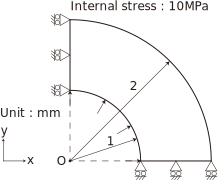
\includegraphics[keepaspectratio, scale = 0.85]
  {fig/内圧を受ける厚肉円筒モデル.ai}
  \caption{Analytical model of thick cylinder subjected to internal pressure}
  \label{fig:internal pressure}
\end{figure}

図~\ref{fig:internal pressure}に示すようにパラメータ空間を設定した.
2次の基底関数を用いた場合と3次の基底関数を用いた場合で,
パラメータ空間の各方向に対してコントロールポイント数が等しく,
一様オープンノットベクトルのIGA解析モデルをそれぞれ作成し,
各方向のコントロールポイントの分割数を変更したIGA解析モデルを作成した.
各方向のコントロールポイント数,自由度数,総要素数を表~\ref{table:ip}に示す.

\begin{table}[hbtp]
  \caption{Details of IGA analytical model}
  \label{table:ip}
  \centering
  \scalebox{0.95}{
    \begin{tabular}{|c|c|c|c|c|c|c|c|c|}
      \hline
      Order of basis function & \multicolumn{4}{c|}{2} & \multicolumn{4}{c|}{3} \\
      \hline
      Control points ($\xi \times \eta$) & $5\times 5$ & $10\times 10$ & $20\times 20$ & $40\times 40$ & $5\times 5$ & $10\times 10$ & $20\times 20$ & $40\times 40$ \\
      \hline
      Degrees of freedom & 40 & 180 & 760 & 3120 & 40 & 180 & 760 & 3120 \\
      \hline
      Total elements & 9 & 64 & 324 & 1444 & 4 & 49 & 289 & 1369 \\
      \hline
    \end{tabular}
  }
\end{table}

\newpage

例として,2次の基底関数と3次の基底関数で,各方向のコントロールポイント数が$5\times 5$のIGA解析モデルを
図~\ref{fig:iga order 2}及び図~\ref{fig:iga order 3}に示す.
点がコントロールポイント,実線が要素境界を表しており,
一様オープンノットベクトルを用いているため,各方向に等間隔の要素分割となっている.

\begin{figure}[htbp]
  \begin{tabular}{cc}
    \begin{minipage}[t]{0.45\hsize}
      \centering
      \includegraphics[keepaspectratio, scale=0.3]
      {fig/result_data_etc/iga/order2/model.png}
      \caption{An example of second-order analytical model (Control points $5\times 5$)}
      \label{fig:iga order 2}
    \end{minipage} &
    \begin{minipage}[t]{0.45\hsize}
      \centering
      \includegraphics[keepaspectratio, scale=0.3]
      {fig/result_data_etc/iga/order3/model.png}
      \caption{An example of third-order analytical model (Control points $5\times 5$)}
      \label{fig:iga order 3}
    \end{minipage}
  \end{tabular}
\end{figure}

\noindent
以上の解析モデルについて解析を行い,精度検証を行った.

内圧$P\ $MPaを受ける内径$2r_1\ $mm,外径$2r_2\ $mmの厚肉円筒の
応力の理論解は,円筒の中心を原点とした極座標表記で以下のように表される.

\begin{align}
  \sigma_{rr} &= -\frac{{r_1}^2{r_2}^2P}{{r_2}^2-{r_1}^2}\frac{1}{r^2}
              +\frac{{r_1}^2P}{{r_2}^2-{r_1}^2}\\
  \sigma_{\theta\theta} &= \frac{{r_1}^2{r_2}^2P}{{r_2}^2-{r_1}^2}\frac{1}{r^2}
                   +\frac{{r_1}^2P}{{r_2}^2-{r_1}^2}
\end{align}

\noindent
この理論解を用いて解析結果の誤差ノルムを算出し,
誤差精度の比較を行った.
誤差ノルムは以下のように定義した.

\begin{equation}
  {\rm{Error\ norm}} = \frac{\sqrt{\int_{\Omega}(\alpha_{\rm{analysis}}-\alpha_{\rm{theory}})^2 d\Omega}}{\sqrt{\int_{\Omega}{\alpha_{\rm{theory}}}^2 d\Omega}}
\end{equation}

\noindent
ここで,$\Omega$はIGA解析モデル全体の領域,
$\alpha$は比較パラメータである半径方向応力$\sigma_{rr}$,周方向応力$\sigma_{\theta\theta}$であり,
$\alpha_{\rm{theory}}$は比較パラメータの理論解,$\alpha_{\rm{analysis}}$は比較パラメータの解析結果の数値を表している.

\newpage

IGA解析結果の変位分布図を示す.
図~\ref{fig:iga 01}~図~\ref{fig:iga 04}は2次の基底関数と3次の基底関数の半径方向変位$u_{r}$である.

\begin{figure}[htbp]
  \begin{tabular}{cc}
    \begin{minipage}[t]{0.45\hsize}
      \centering
      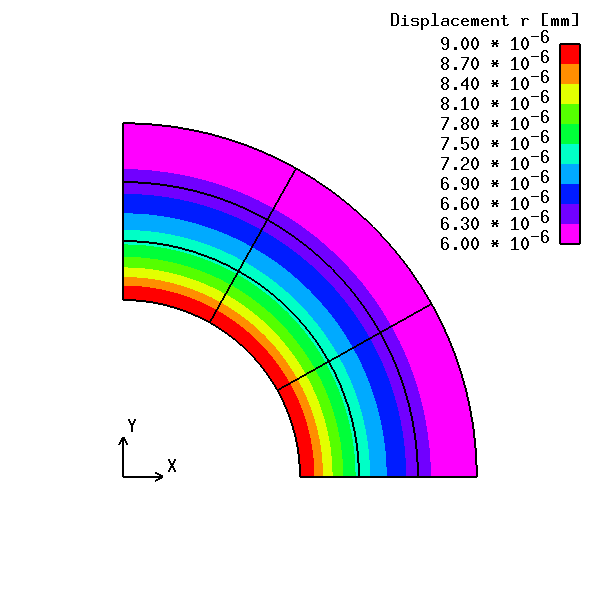
\includegraphics[keepaspectratio, scale=0.3]
      {fig/result_data_etc/iga/order2/2_5x5.png}
      \caption{Displacement in r direction of second-order analytical model (Control points $5\times 5$)}
      \label{fig:iga 01}
    \end{minipage} &
    \begin{minipage}[t]{0.45\hsize}
      \centering
      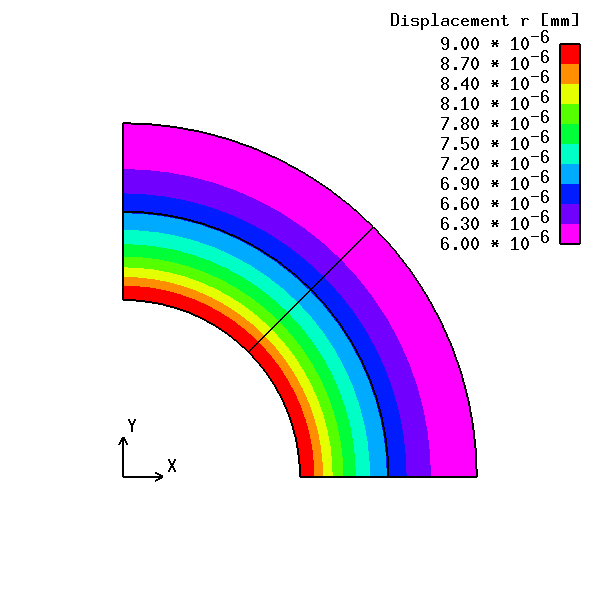
\includegraphics[keepaspectratio, scale=0.3]
      {fig/result_data_etc/iga/order3/3_5x5.png}
      \caption{Displacement in r direction of third-order analytical model (Control points $5\times 5$)}
      \label{fig:iga 02}
    \end{minipage}
  \end{tabular}
\end{figure}

\begin{figure}[htbp]
  \begin{tabular}{cc}
    \begin{minipage}[t]{0.45\hsize}
      \centering
      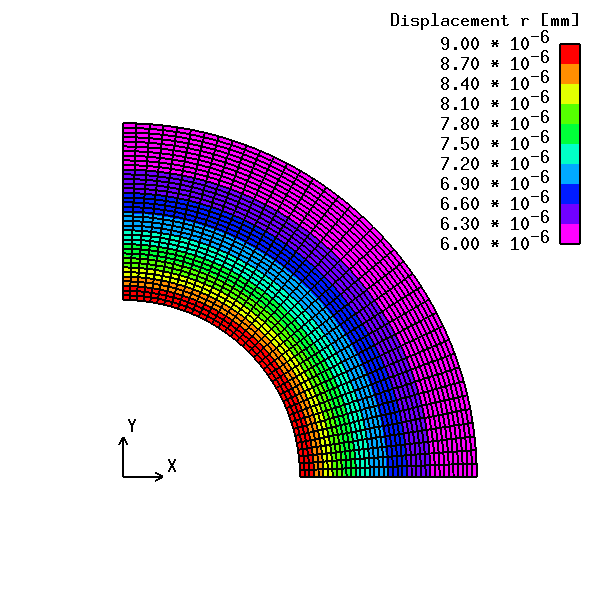
\includegraphics[keepaspectratio, scale=0.3]
      {fig/result_data_etc/iga/order2/2_40x40.png}
      \caption{Displacement in r direction of second-order analytical model (Control points $40\times 40$)}
      \label{fig:iga 03}
    \end{minipage} &
    \begin{minipage}[t]{0.45\hsize}
      \centering
      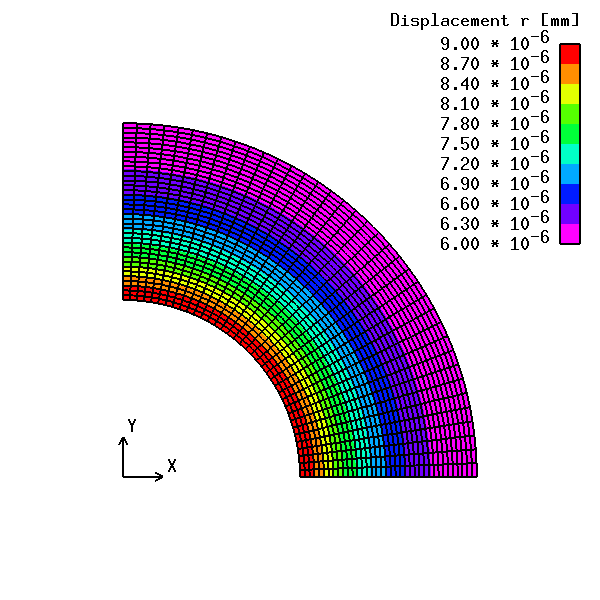
\includegraphics[keepaspectratio, scale=0.3]
      {fig/result_data_etc/iga/order3/3_40x40.png}
      \caption{Displacement in r direction of third-order analytical model (Control points $40\times 40$)}
      \label{fig:iga 04}
    \end{minipage}
  \end{tabular}
\end{figure}

半径方向応力$\sigma_{rr}$と周方向応力$\sigma_{\theta\theta}$の誤差ノルムを算出し,
2次の基底関数を用いた場合と3次の基底関数を用いた場合の
自由度数と誤差ノルムの関係を両対数グラフで図~\ref{fig:iga ER 01},図~\ref{fig:iga ER 02}に示す.

\begin{figure}[htbp]
  \centering
  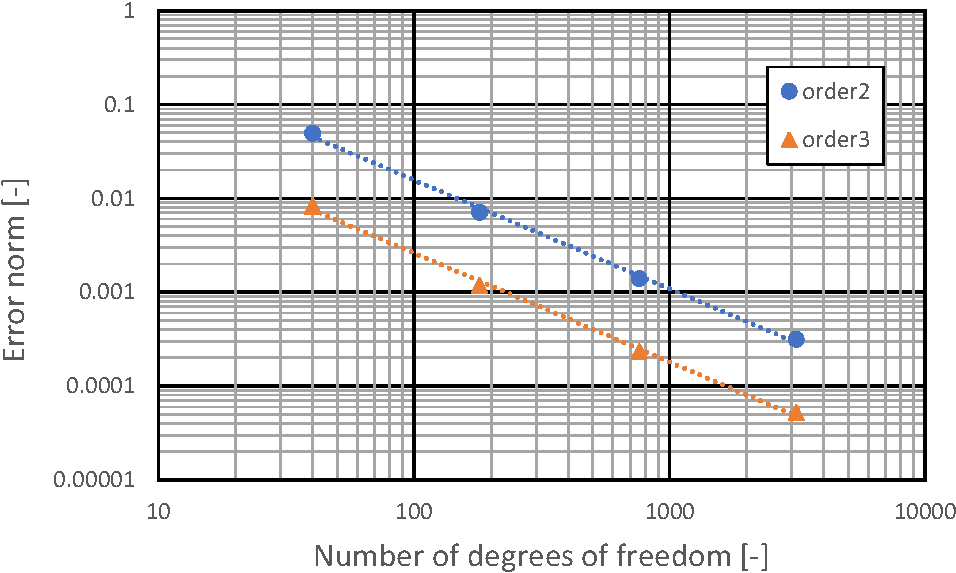
\includegraphics[keepaspectratio, scale = 0.8]
  {fig/result_data_etc/iga/ER01-crop.pdf}
  \caption{Error norm of $\sigma_{rr}$}
  \label{fig:iga ER 01}
\end{figure}

\begin{figure}[htbp]
  \centering
  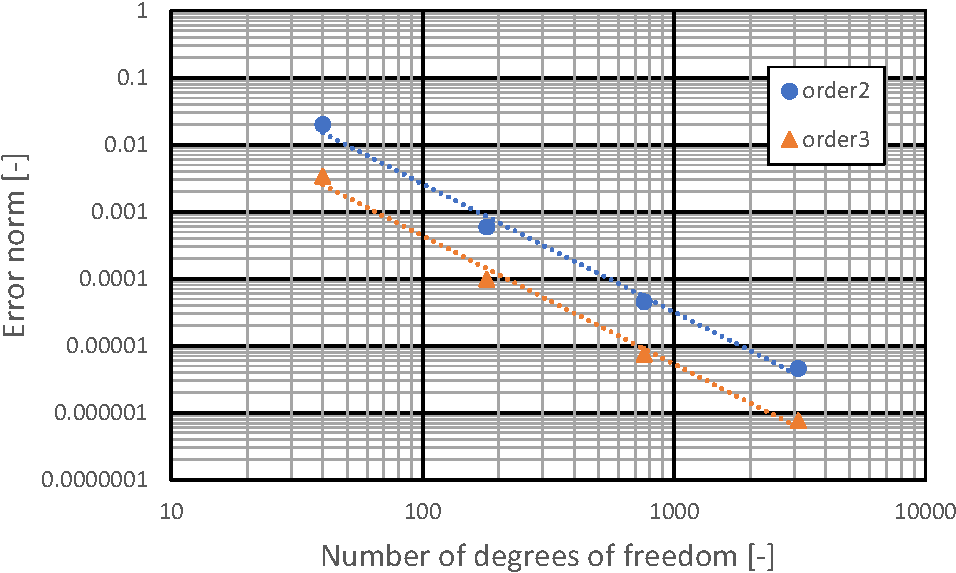
\includegraphics[keepaspectratio, scale = 0.8]
  {fig/result_data_etc/iga/ER02-crop.pdf}
  \caption{Error norm of $\sigma_{\theta\theta}$}
  \label{fig:iga ER 02}
\end{figure}

\newpage

\section{3次の基底関数を用いた重合パッチ法解析}
重合パッチ法解析を行い,2次と
3次の基底関数を用いた解析の誤差精度の検証を行った.

\subsection{遠方で一様引張を受ける円孔を有する平板の解析}

解析対象は,中央に半径$1\ $mmの円孔を有する遠方で一様引張を受ける平板であり,解析には二次元の$1/4$モデルを使用した.
解析問題を図~\ref{fig:GL}に示す.
平面ひずみ状態を仮定し,ヤング率は$206\ $GPa,ポアソン比は$0.3$とした.

\begin{figure}[htbp]
  \centering
  \includegraphics[keepaspectratio, scale = 0.85]
  {fig/GL.ai}
  \caption{Analytical model of plate with a circular hole}
  \label{fig:GL}
\end{figure}

\noindent
図~\ref{fig:GL}の問題は重合パッチ法では図~\ref{fig:G_and_L}に示す解析モデルと等価である.

\begin{figure}[htbp]
  \centering
  \includegraphics[keepaspectratio, scale = 0.85]
  {fig/G_and_L.ai}
  \caption{Analytical model of Global patch and Local patch}
  \label{fig:G_and_L}
\end{figure}

\newpage

\noindent
グローバルパッチはシンプルな形状を作成し,一様引張と対称性を表すための変位固定の境界条件を設定した.
ローカルパッチは円孔を表現する詳細形状を作成し,グローバルパッチ上のローカルパッチの境界$\Gamma^{GL}$で変位固定を行った.

数値積分には各方向の積分点数が$4\times 4$のガウス・ルジャンドル積分法を用いた.
ただし,ローカルパッチの1要素がグローバルパッチの2要素以上を跨ぐ場合では
被積分関数がグローバルパッチの要素境界で連続性が低下し,
結合剛性マトリクスの積分精度が低下することが確認されており,
該当するローカルパッチについては積分点数を$10\times 10$として積分を行った.

図~\ref{fig:G_and_L}に示すようにパラメータ空間を設定した.
ノットベクトルは一様オープンノットベクトルを用いた.

無限遠にて一様引張応力$\sigma_0$を受ける場合の理論解は円孔の中心を原点とする極座標表記を用いて以下のように表される.

\begin{align}
  \sigma_{rr} &= \frac{\sigma_0}{2}\left(1 - \frac{\rho^2}{r^2}\right) - \frac{\sigma_0}{2}\left(1 - \frac{4\rho^2}{r^2} + \frac{3\rho^4}{r^4}\right)\cos{2\theta}\\
  \sigma_{\theta\theta} &= \frac{\sigma_0}{2}\left(1 + \frac{\rho^2}{r^2}\right) + \frac{\sigma_0}{2} \left( 1 + \frac{3\rho^4}{r^4} \right) \cos{2\theta}\\
  \tau_{r\theta} &= \frac{\sigma_0}{2} \left( 1 + \frac{2\rho^2}{r^2} - \frac{3\rho^4}{r^4} \right)
\end{align}

\noindent
また,直交座標系から極座標系への座標変換は以下のように表される.

\begin{align}
  \sigma_{rr} &= \sigma_{xx} \cos^2\theta + \sigma_{yy} \sin^2\theta + 2\tau_{xy} \sin\theta \cos\theta \\
  \sigma_{\theta\theta} &= \sigma_{xx} \sin^2\theta + \sigma_{yy} \cos^2\theta - 2\tau_{xy} \cos\theta \sin\theta \\
  \tau_{r\theta} &= (\sigma_{yy} - \sigma_{xx}) \sin\theta \cos\theta + \tau_{xy}(\cos^2\theta - \sin^2\theta)
\end{align}

\noindent
この理論解を用いて解析結果の誤差ノルムを以下のように定義する.

\begin{equation}
  {\rm{Error\ norm}} = \frac{\sqrt{\int_{\Omega^L}(\alpha_{\rm{analysis}}-\alpha_{\rm{theory}})^2 d\Omega}}{\sqrt{\int_{\Omega^L}{\alpha_{\rm{theory}}}^2 d\Omega}}
\end{equation}

\noindent
ここで,$\Omega^L$は重合パッチ法解析モデルにおけるローカルパッチの領域,
$\alpha$は比較パラメータである半径方向応力$\sigma_{rr}$,周方向応力$\sigma_{\theta\theta}$であり,
$\alpha_{\rm{theory}}$は比較パラメータの理論解,$\alpha_{\rm{analysis}}$は比較パラメータの解析結果の数値を表している.

\subsubsection{各パッチでの基底関数の次数の組み合わせによる解析精度検証}
表~\ref{table:combination}に示すようにグローバルパッチとローカルパッチをそれぞれ2次の基底関数,3次の基底関数で作成し,
その組み合わせの違いによる誤差精度を検証した.
さらに表~\ref{table:GL_division}に示すように各組み合わせでグローバルパッチの分割数を固定して,ローカルパッチの分割数を変更した.

\begin{table}[hbtp]
  \caption{Combination of order of basis function}
  \label{table:combination}
  \centering
  \scalebox{1.0}{
    \begin{tabular}{|c|c|c|}
      \hline
       &
      \begin{tabular}{c}
        Order of basis function \\
        on Global patch
      \end{tabular} &
      \begin{tabular}{c}
        Order of basis function \\
        on Local patch
      \end{tabular} \\
      \hline
      (a) Order(2, 2) & 2 & 2 \\
      \hline
      (b) Order(2, 3) & 2 & 3 \\
      \hline
      (c) Order(3, 2) & 3 & 2 \\
      \hline
      (d) Order(3, 3) & 3 & 3 \\
      \hline
    \end{tabular}
  }
\end{table}

\begin{table}[hbtp]
  \caption{Control points on Global patch and Local patch}
  \label{table:GL_division}
  \centering
  \scalebox{1.0}{
    \begin{tabular}{|c|c|c|c|c|}
      \hline
      \begin{tabular}{c}
        Control points\\
        on Global patch ($\xi \times \eta$)
      \end{tabular} & \multicolumn{4}{c|}{$30\times 30$} \\
      \hline
      \begin{tabular}{c}
        Control points\\
        on Local patch ($\xi \times \eta$)
      \end{tabular} & $5\times 5$ & $10\times 10$ & $20\times 20$ & $30\times 30$ \\
      \hline
    \end{tabular}
  }
\end{table}

例として,各組み合わせでローカルパッチの各方向のコントロールポイント数が$5\times 5$の重合パッチ法解析モデルを
図~\ref{fig:22}及び図~\ref{fig:33}に示す.

\begin{figure}[htbp]
  \begin{tabular}{cc}
    \begin{minipage}[t]{0.45\hsize}
      \centering
      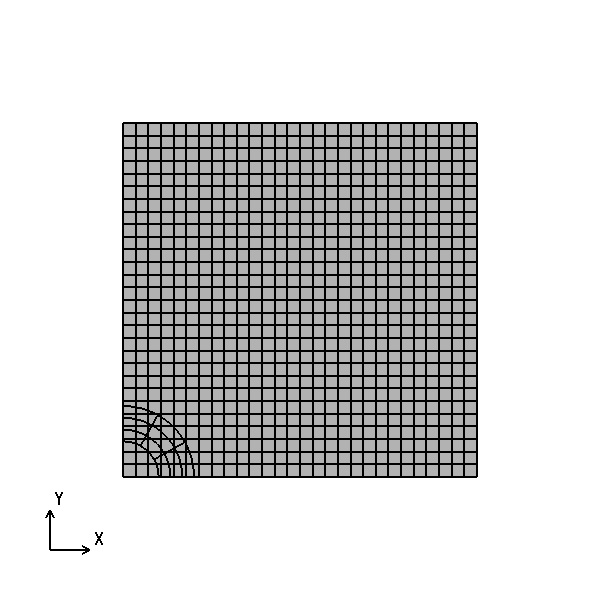
\includegraphics[keepaspectratio, scale=0.3]
      {fig/result_data_etc/s-iga01/model/22.png}
      \caption{An example of (a) analytical model (Order(2, 2), Control points on Local patch $5\times 5$)}
      \label{fig:22}
    \end{minipage} &
    \begin{minipage}[t]{0.45\hsize}
      \centering
      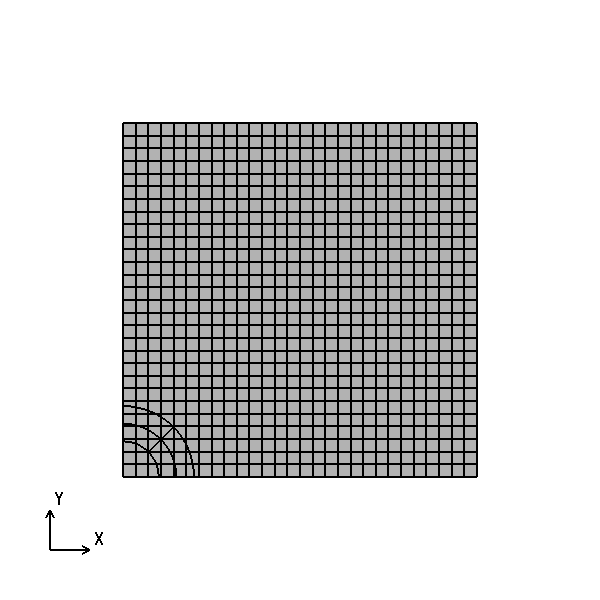
\includegraphics[keepaspectratio, scale=0.3]
      {fig/result_data_etc/s-iga01/model/23.png}
      \caption{An example of (b) analytical model (Order(2, 3), Control points on Local patch $5\times 5$)}
      \label{fig:23}
    \end{minipage}
  \end{tabular}
\end{figure}

\newpage

\begin{figure}[htbp]
  \begin{tabular}{cc}
    \begin{minipage}[t]{0.45\hsize}
      \centering
      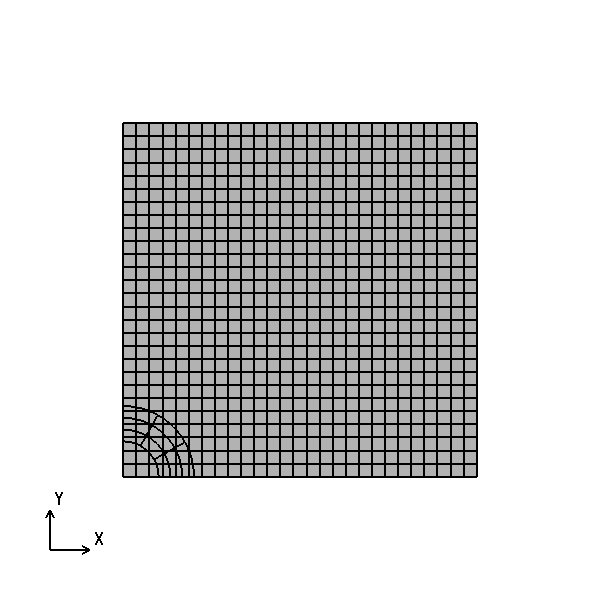
\includegraphics[keepaspectratio, scale=0.3]
      {fig/result_data_etc/s-iga01/model/32.png}
      \caption{An example of (c) analytical model (Order(3, 2), Control points on Local patch $5\times 5$)}
      \label{fig:32}
    \end{minipage} &
    \begin{minipage}[t]{0.45\hsize}
      \centering
      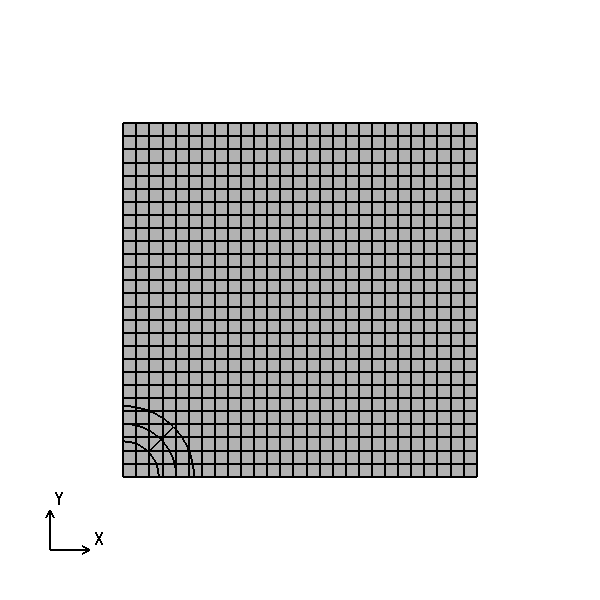
\includegraphics[keepaspectratio, scale=0.3]
      {fig/result_data_etc/s-iga01/model/33.png}
      \caption{An example of (d) analytical model (Order(3, 3), Control points on Local patch $5\times 5$)}
      \label{fig:33}
    \end{minipage}
  \end{tabular}
\end{figure}

\noindent
以上の解析モデルについて解析を行い,精度検証を行った.
半径方向応力$\sigma_{rr}$と周方向応力$\sigma_{\theta\theta}$の自由度と誤差ノルムの関係を
図~\ref{fig:ERNr},図~\ref{fig:ERNt}に示す.

\begin{figure}[htbp]
  \centering
  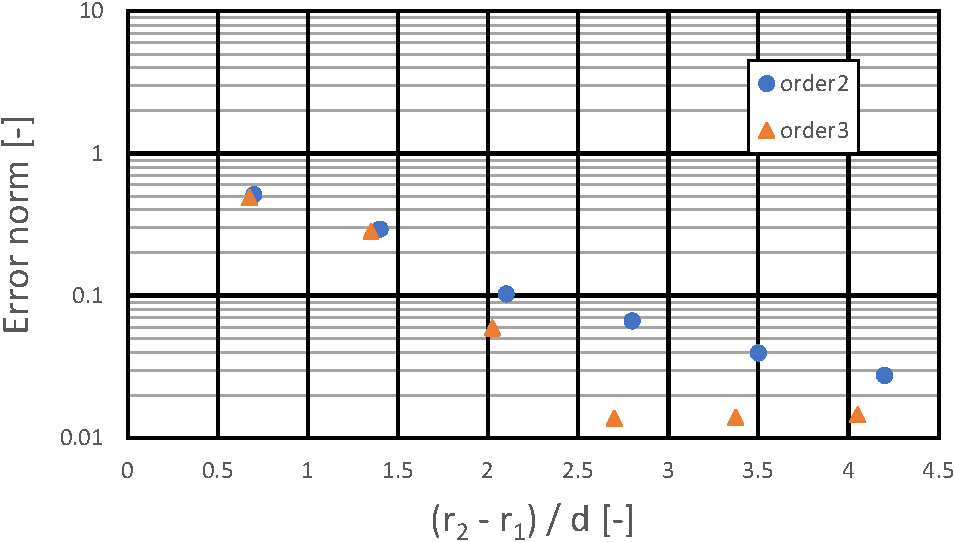
\includegraphics[keepaspectratio, scale=0.5]
  {fig/result_data_etc/s-iga01/r-crop.pdf}
  \caption{Error norm of $\sigma_{rr}$ in each case}
  \label{fig:ERNr}
\end{figure}

\newpage

\begin{figure}[htbp]
  \centering
  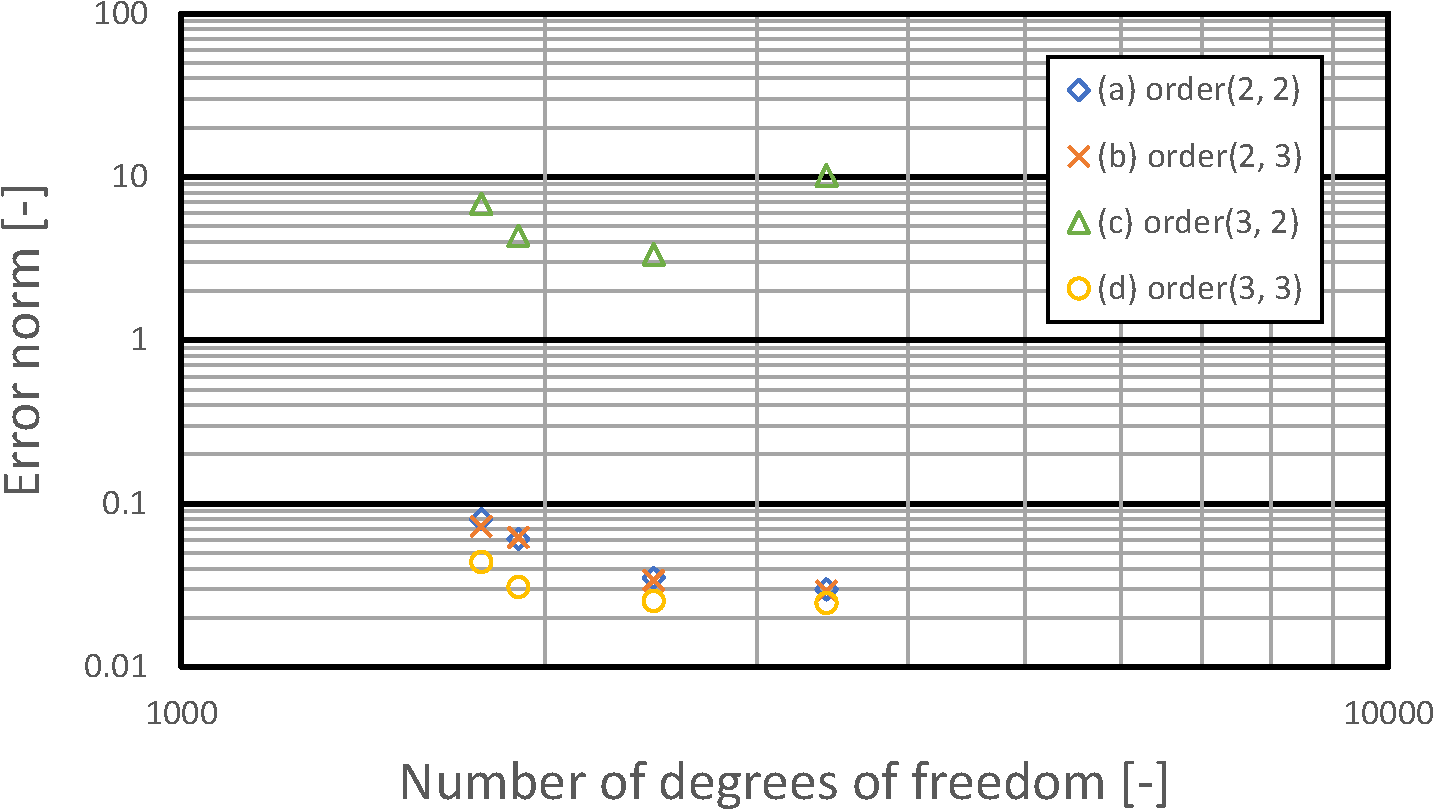
\includegraphics[keepaspectratio, scale=0.5]
  {fig/result_data_etc/s-iga01/theta-crop.pdf}
  \caption{Error norm of $\sigma_{\theta\theta}$ in each case}
  \label{fig:ERNt}
\end{figure}

$y$方向応力$\sigma_{yy}$の応力分布図を図~\ref{fig:contour22}~図~\ref{fig:contour33}に示す.

\begin{figure}[htbp]
  \begin{tabular}{cc}
    \begin{minipage}[t]{0.45\hsize}
      \centering
      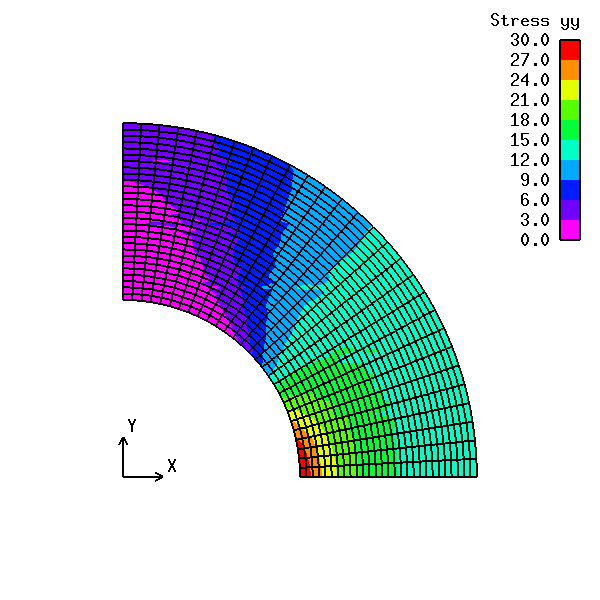
\includegraphics[keepaspectratio, scale=0.3]
      {fig/result_data_etc/s-iga01/contour/2_2.png}
      \caption{Stress in $y$ direction on Local patch ((a) Order(2, 2), Control points on Local patch $30\times 30$)}
      \label{fig:contour22}
    \end{minipage} &
    \begin{minipage}[t]{0.45\hsize}
      \centering
      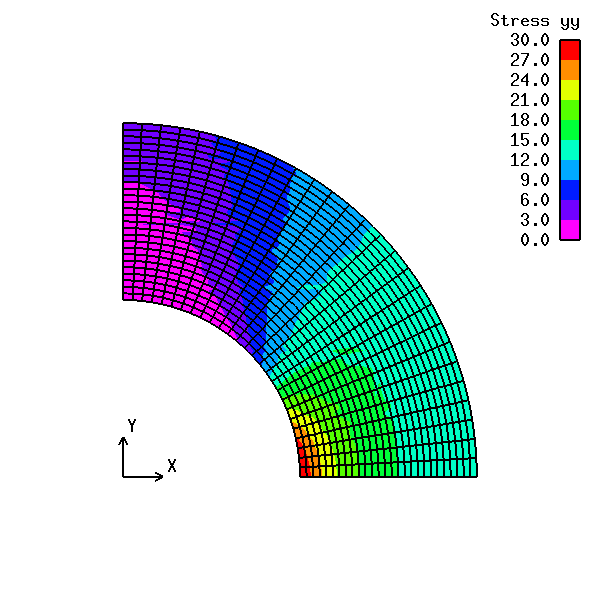
\includegraphics[keepaspectratio, scale=0.3]
      {fig/result_data_etc/s-iga01/contour/2_3.png}
      \caption{Stress in $y$ direction on Local patch ((b) Order(2, 3), Control points on Local patch $30\times 30$)}
      \label{fig:contour23}
    \end{minipage}
  \end{tabular}
\end{figure}

\newpage

\begin{figure}[htbp]
  \begin{tabular}{cc}
    \begin{minipage}[t]{0.45\hsize}
      \centering
      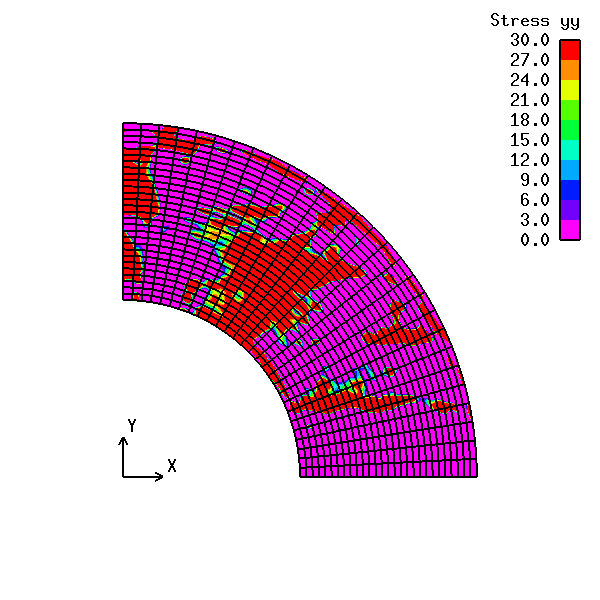
\includegraphics[keepaspectratio, scale=0.3]
      {fig/result_data_etc/s-iga01/contour/3_2.png}
      \caption{Stress in $y$ direction on Local patch ((c) Order(3, 2), Control points on Local patch $30\times 30$)}
      \label{fig:contour32}
    \end{minipage} &
    \begin{minipage}[t]{0.45\hsize}
      \centering
      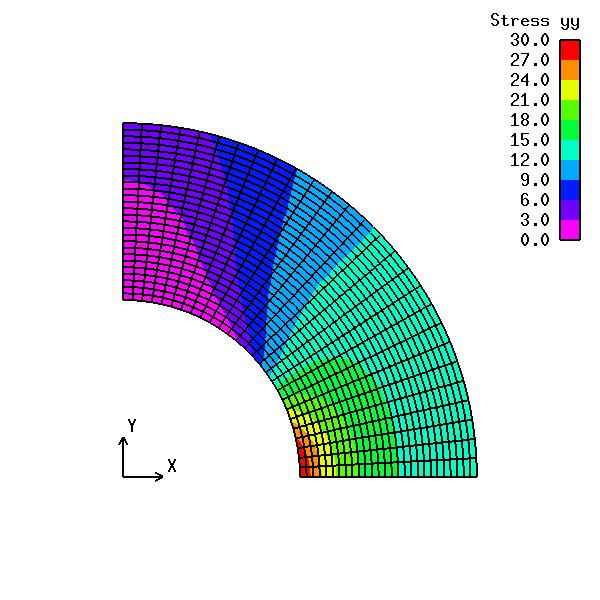
\includegraphics[keepaspectratio, scale=0.3]
      {fig/result_data_etc/s-iga01/contour/3_3.png}
      \caption{Stress in $y$ direction on Local patch ((d) Order(3, 3), Control points on Local patch $30\times 30$)}
      \label{fig:contour33}
    \end{minipage}
  \end{tabular}
\end{figure}

\newpage

\subsubsection{グローバルパッチの分割数を固定してローカルパッチの分割数を変更した解析}
グローバルパッチのコントロールポイントの分割数を固定してローカルパッチのコントロールポイントの分割数を
変更した重合パッチ法解析を行った.
グローバルパッチとローカルパッチの基底関数が共に2次の場合と共に3次の場合で解析を行い比較した.
グローバルパッチとローカルパッチは
2次の基底関数を用いた場合と3次の基底関数を用いた場合で,
パラメータ空間の各方向に対してコントロールポイント数が等しく,
各方向のコントロールポイントの分割数を変更した重合パッチ法解析モデルを作成した.
グローバルパッチとローカルパッチの各方向のコントロールポイント数,自由度数,総要素数を表~\ref{table:G fixed}に示す.

\begin{table}[hbtp]
  \caption{Details of S-IGA analytical model (Global patch division is fixed)}
  \label{table:G fixed}
  \centering
  \scalebox{0.8}{
    \begin{tabular}{|c|c|c|c|c|c|c|c|c|}
      \hline
      \begin{tabular}{c}
        Order of basis function \\
        (Global patch and Local patch)
      \end{tabular} & \multicolumn{4}{c|}{2} & \multicolumn{4}{c|}{3} \\
      \hline
      \begin{tabular}{c}
        Control points\\
        on Global patch ($\xi \times \eta$)
      \end{tabular} & \multicolumn{4}{c|}{$30\times 30$} & \multicolumn{4}{c|}{$30\times 30$} \\
      \hline
      \begin{tabular}{c}
        Control points\\
        on Local patch ($\xi \times \eta$)
      \end{tabular} & $5\times 5$ & $10\times 10$ & $20\times 20$ & $30\times 30$ & $5\times 5$ & $10\times 10$ & $20\times 20$ & $30\times 30$ \\
      \hline
      Degrees of freedom & 1772 & 1902 & 2462 & 3422 & 1772 & 1902 & 2462 & 3422 \\
      \hline
      Total elements & 793 & 848 & 1108 & 1568 & 733 & 778 & 1018 & 1458 \\
      \hline
    \end{tabular}
  }
\end{table}

例として,2次の基底関数で,ローカルパッチの分割数を変更した重合パッチ法解析モデルを図~\ref{fig:s-iga02 model01}~
図~\ref{fig:s-iga02 model04}に示す.

\begin{figure}[htbp]
  \begin{tabular}{cc}
    \begin{minipage}[t]{0.45\hsize}
      \centering
      \includegraphics[keepaspectratio, scale=0.3]
      {fig/result_data_etc/s-iga02/model/5x5.png}
      \caption{An example of second-order S-IGA analytical model (Global patch $30\times 30$, Local patch $5\times 5$)}
      \label{fig:s-iga02 model01}
    \end{minipage} &
    \begin{minipage}[t]{0.45\hsize}
      \centering
      \includegraphics[keepaspectratio, scale=0.3]
      {fig/result_data_etc/s-iga02/model/10x10.png}
      \caption{An example of second-order S-IGA analytical model (Global patch $30\times 30$, Local patch $10\times 10$)}
      \label{fig:s-iga02 model02}
    \end{minipage}
  \end{tabular}
\end{figure}

\newpage

\begin{figure}[hbtp]
  \begin{tabular}{cc}
    \begin{minipage}[t]{0.45\hsize}
      \centering
      \includegraphics[keepaspectratio, scale=0.3]
      {fig/result_data_etc/s-iga02/model/20x20.png}
      \caption{An example of second-order S-IGA analytical model (Global patch $30\times 30$, Local patch $20\times 20$)}
      \label{fig:s-iga02 model03}
    \end{minipage} &
    \begin{minipage}[t]{0.45\hsize}
      \centering
      \includegraphics[keepaspectratio, scale=0.3]
      {fig/result_data_etc/s-iga02/model/30x30.png}
      \caption{An example of second-order S-IGA analytical model (Global patch $30\times 30$, Local patch $30\times 30$)}
      \label{fig:s-iga02 model04}
    \end{minipage}
  \end{tabular}
\end{figure}

\noindent
以上の解析モデルについて解析を行い,精度検証を行った.
円孔縁の主応力$\sigma_1, \sigma_2$の分布,$x$軸上の$y$方向応力$\sigma_{yy}$,応力分布図を比較し,
ローカルパッチの分割数による影響を比較した.

円孔縁の主応力$\sigma_1, \sigma_2$の分布を
図~\ref{fig:s-iga02 s 2 5x5}~図~\ref{fig:s-iga02 s 3 30x30}に示す.

\begin{figure}[hbtp]
  \begin{tabular}{cc}
    \begin{minipage}[t]{0.45\hsize}
      \centering
      \includegraphics[keepaspectratio, scale=0.4]
      {fig/result_data_etc/s-iga02/order2/s_5x5-crop.pdf}
      \caption{Principal stress along the periphery of the circular hole (second-order, Global patch $30\times 30$, Local patch $5\times 5$)}
      \label{fig:s-iga02 s 2 5x5}
    \end{minipage} &
    \begin{minipage}[t]{0.45\hsize}
      \centering
      \includegraphics[keepaspectratio, scale=0.4]
      {fig/result_data_etc/s-iga02/order3/s_5x5-crop.pdf}
      \caption{Principal stress along the periphery of the circular hole (third-order, Global patch $30\times 30$, Local patch $5\times 5$)}
      \label{fig:s-iga02 s 3 5x5}
    \end{minipage}
  \end{tabular}
\end{figure}

\newpage

\begin{figure}[hbtp]
  \begin{tabular}{cc}
    \begin{minipage}[t]{0.45\hsize}
      \centering
      \includegraphics[keepaspectratio, scale=0.4]
      {fig/result_data_etc/s-iga02/order2/s_10x10-crop.pdf}
      \caption{Principal stress along the periphery of the circular hole (second-order, Global patch $30\times 30$, Local patch $10\times 10$)}
      \label{fig:s-iga02 s 2 10x10}
    \end{minipage} &
    \begin{minipage}[t]{0.45\hsize}
      \centering
      \includegraphics[keepaspectratio, scale=0.4]
      {fig/result_data_etc/s-iga02/order3/s_10x10-crop.pdf}
      \caption{Principal stress along the periphery of the circular hole (third-order, Global patch $30\times 30$, Local patch $10\times 10$)}
      \label{fig:s-iga02 s 3 10x10}
    \end{minipage}
  \end{tabular}
\end{figure}

\begin{figure}[hbtp]
  \begin{tabular}{cc}
    \begin{minipage}[t]{0.45\hsize}
      \centering
      \includegraphics[keepaspectratio, scale=0.4]
      {fig/result_data_etc/s-iga02/order2/s_20x20-crop.pdf}
      \caption{Principal stress along the periphery of the circular hole (second-order, Global patch $30\times 30$, Local patch $20\times 20$)}
      \label{fig:s-iga02 s 2 20x20}
    \end{minipage} &
    \begin{minipage}[t]{0.45\hsize}
      \centering
      \includegraphics[keepaspectratio, scale=0.4]
      {fig/result_data_etc/s-iga02/order3/s_20x20-crop.pdf}
      \caption{Principal stress along the periphery of the circular hole (third-order, Global patch $30\times 30$, Local patch $20\times 20$)}
      \label{fig:s-iga02 s 3 20x20}
    \end{minipage}
  \end{tabular}
\end{figure}

\begin{figure}[hbtp]
  \begin{tabular}{cc}
    \begin{minipage}[t]{0.45\hsize}
      \centering
      \includegraphics[keepaspectratio, scale=0.4]
      {fig/result_data_etc/s-iga02/order2/s_30x30-crop.pdf}
      \caption{Principal stress along the periphery of the circular hole (second-order, Global patch $30\times 30$, Local patch $30\times 30$)}
      \label{fig:s-iga02 s 2 30x30}
    \end{minipage} &
    \begin{minipage}[t]{0.45\hsize}
      \centering
      \includegraphics[keepaspectratio, scale=0.4]
      {fig/result_data_etc/s-iga02/order3/s_30x30-crop.pdf}
      \caption{Principal stress along the periphery of the circular hole (third-order, Global patch $30\times 30$, Local patch $30\times 30$)}
      \label{fig:s-iga02 s 3 30x30}
    \end{minipage}
  \end{tabular}
\end{figure}

\newpage

$x$軸上の$y$方向応力$\sigma_{yy}$を
図~\ref{fig:s-iga02 y 2 5x5}~図~\ref{fig:s-iga02 y 3 30x30}に示す.

\begin{figure}[hbtp]
  \begin{tabular}{cc}
    \begin{minipage}[t]{0.45\hsize}
      \centering
      \includegraphics[keepaspectratio, scale=0.4]
      {fig/result_data_etc/s-iga02/order2/y_5x5-crop.pdf}
      \caption{Stress in $y$ direction along the line $y = 0$ (second-order, Global patch $30\times 30$, Local patch $5\times 5$)}
      \label{fig:s-iga02 y 2 5x5}
    \end{minipage} &
    \begin{minipage}[t]{0.45\hsize}
      \centering
      \includegraphics[keepaspectratio, scale=0.4]
      {fig/result_data_etc/s-iga02/order3/y_5x5-crop.pdf}
      \caption{Stress in $y$ direction along the line $y = 0$ (third-order, Global patch $30\times 30$, Local patch $5\times 5$)}
      \label{fig:s-iga02 y 3 5x5}
    \end{minipage}
  \end{tabular}
\end{figure}

\begin{figure}[hbtp]
  \begin{tabular}{cc}
    \begin{minipage}[t]{0.45\hsize}
      \centering
      \includegraphics[keepaspectratio, scale=0.4]
      {fig/result_data_etc/s-iga02/order2/y_10x10-crop.pdf}
      \caption{Stress in $y$ direction along the line $y = 0$ (second-order, Global patch $30\times 30$, Local patch $10\times 10$)}
      \label{fig:s-iga02 y 2 10x10}
    \end{minipage} &
    \begin{minipage}[t]{0.45\hsize}
      \centering
      \includegraphics[keepaspectratio, scale=0.4]
      {fig/result_data_etc/s-iga02/order3/y_10x10-crop.pdf}
      \caption{Stress in $y$ direction along the line $y = 0$ (third-order, Global patch $30\times 30$, Local patch $10\times 10$)}
      \label{fig:s-iga02 y 3 10x10}
    \end{minipage}
  \end{tabular}
\end{figure}

\begin{figure}[hbtp]
  \begin{tabular}{cc}
    \begin{minipage}[t]{0.45\hsize}
      \centering
      \includegraphics[keepaspectratio, scale=0.4]
      {fig/result_data_etc/s-iga02/order2/y_20x20-crop.pdf}
      \caption{Stress in $y$ direction along the line $y = 0$ (second-order, Global patch $30\times 30$, Local patch $20\times 20$)}
      \label{fig:s-iga02 y 2 20x20}
    \end{minipage} &
    \begin{minipage}[t]{0.45\hsize}
      \centering
      \includegraphics[keepaspectratio, scale=0.4]
      {fig/result_data_etc/s-iga02/order3/y_20x20-crop.pdf}
      \caption{Stress in $y$ direction along the line $y = 0$ (third-order, Global patch $30\times 30$, Local patch $20\times 20$)}
      \label{fig:s-iga02 y 3 20x20}
    \end{minipage}
  \end{tabular}
\end{figure}

\newpage

\begin{figure}[hbtp]
  \begin{tabular}{cc}
    \begin{minipage}[t]{0.45\hsize}
      \centering
      \includegraphics[keepaspectratio, scale=0.4]
      {fig/result_data_etc/s-iga02/order2/y_30x30-crop.pdf}
      \caption{Stress in $y$ direction along the line $y = 0$ (second-order, Global patch $30\times 30$, Local patch $30\times 30$)}
      \label{fig:s-iga02 y 2 30x30}
    \end{minipage} &
    \begin{minipage}[t]{0.45\hsize}
      \centering
      \includegraphics[keepaspectratio, scale=0.4]
      {fig/result_data_etc/s-iga02/order3/y_30x30-crop.pdf}
      \caption{Stress in $y$ direction along the line $y = 0$ (third-order, Global patch $30\times 30$, Local patch $30\times 30$)}
      \label{fig:s-iga02 y 3 30x30}
    \end{minipage}
  \end{tabular}
\end{figure}

$y$方向応力$\sigma_{yy}$の分布図を図~\ref{fig:s-iga02 y 2},図~\ref{fig:s-iga02 y 3}に示す.

\begin{figure}[hbtp]
  \begin{tabular}{cc}
    \begin{minipage}[t]{0.45\hsize}
      \centering
      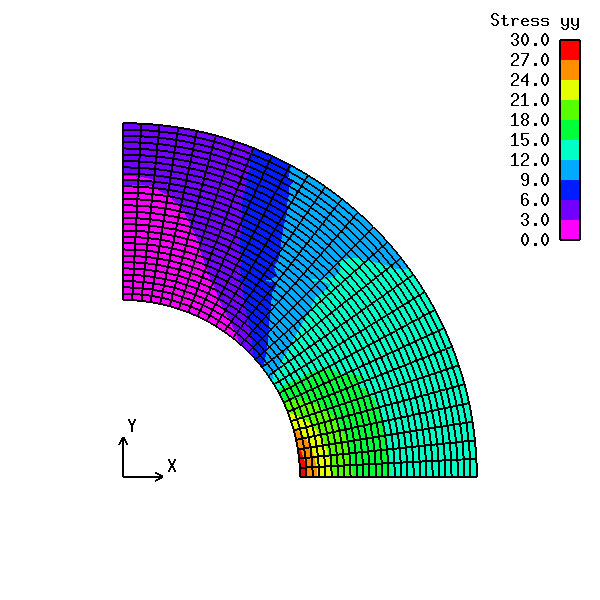
\includegraphics[keepaspectratio, scale=0.3]
      {fig/result_data_etc/s-iga02/contour/2.png}
      \caption{Stress in $y$ direction on Local patch (second-order, Global patch $30\times 30$, Local patch $20\times 20$)}
      \label{fig:s-iga02 y 2}
    \end{minipage} &
    \begin{minipage}[t]{0.45\hsize}
      \centering
      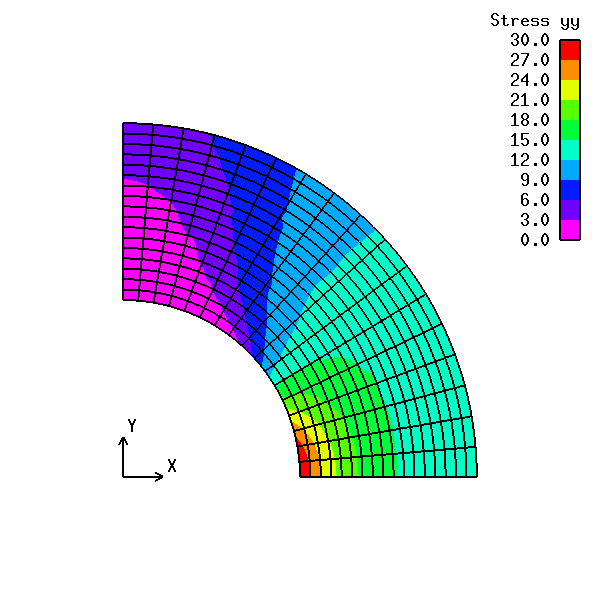
\includegraphics[keepaspectratio, scale=0.3]
      {fig/result_data_etc/s-iga02/contour/3.png}
      \caption{Stress in $y$ direction on Local patch (third-order, Global patch $30\times 30$, Local patch $20\times 20$)}
      \label{fig:s-iga02 y 3}
    \end{minipage}
  \end{tabular}
\end{figure}

\newpage

\subsubsection{ローカルパッチの分割数を固定してグローバルパッチの分割数を変更した解析}
ローカルパッチのコントロールポイントの分割数を固定してグローバルパッチのコントロールポイントの分割数を
変更した重合パッチ法解析を行った.
グローバルパッチとローカルパッチの基底関数が共に2次の場合と共に3次の場合で解析を行い比較した.
グローバルパッチとローカルパッチは
2次の基底関数を用いた場合と3次の基底関数を用いた場合で,
パラメータ空間の各方向に対してコントロールポイント数が等しく,
各方向のコントロールポイントの分割数を変更した重合パッチ法解析モデルを作成した.
グローバルパッチとローカルパッチの各方向のコントロールポイント数,自由度数,総要素数を表~\ref{table:L fixed}に示す.

\begin{table}[hbtp]
  \caption{Details of S-IGA analytical model (Local patch division is fixed)}
  \label{table:L fixed}
  \centering
  \scalebox{0.8}{
    \begin{tabular}{|c|c|c|c|c|c|c|c|c|}
      \hline
      \begin{tabular}{c}
        Order of basis function \\
        (Global patch and Local patch)
      \end{tabular} & \multicolumn{4}{c|}{2} & \multicolumn{4}{c|}{3} \\
      \hline
      \begin{tabular}{c}
        Control points\\
        on Local patch ($\xi \times \eta$)
      \end{tabular} & \multicolumn{4}{c|}{$30\times 30$} & \multicolumn{4}{c|}{$30\times 30$} \\
      \hline
      \begin{tabular}{c}
        Control points\\
        on Global patch ($\xi \times \eta$)
      \end{tabular} & $5\times 5$ & $10\times 10$ & $20\times 20$ & $30\times 30$ & $5\times 5$ & $10\times 10$ & $20\times 20$ & $30\times 30$ \\
      \hline
      Degrees of freedom & 1722 & 1862 & 2442 & 3422 & 1722 & 1862 & 2442 & 3422 \\
      \hline
      Total elements & 793 & 848 & 1108 & 1568 & 733 & 778 & 1018 & 1458 \\
      \hline
    \end{tabular}
  }
\end{table}

例として,2次の基底関数で,グローバルパッチの分割数を変更した重合パッチ法解析モデルを図~\ref{fig:s-iga03 model01}~
図~\ref{fig:s-iga03 model04}に示す.

\begin{figure}[htbp]
  \begin{tabular}{cc}
    \begin{minipage}[t]{0.45\hsize}
      \centering
      \includegraphics[keepaspectratio, scale=0.3]
      {fig/result_data_etc/s-iga03/model/5x5.png}
      \caption{An example of second-order S-IGA analytical model (Global patch $5\times 5$, Local patch $30\times 30$)}
      \label{fig:s-iga03 model01}
    \end{minipage} &
    \begin{minipage}[t]{0.45\hsize}
      \centering
      \includegraphics[keepaspectratio, scale=0.3]
      {fig/result_data_etc/s-iga03/model/10x10.png}
      \caption{An example of second-order S-IGA analytical model (Global patch $10\times 10$, Local patch $30\times 30$)}
      \label{fig:s-iga03 model02}
    \end{minipage}
  \end{tabular}
\end{figure}

\newpage

\begin{figure}[htbp]
  \begin{tabular}{cc}
    \begin{minipage}[t]{0.45\hsize}
      \centering
      \includegraphics[keepaspectratio, scale=0.3]
      {fig/result_data_etc/s-iga03/model/20x20.png}
      \caption{An example of second-order S-IGA analytical model (Global patch $20\times 20$, Local patch $30\times 30$)}
      \label{fig:s-iga03 model03}
    \end{minipage} &
    \begin{minipage}[t]{0.45\hsize}
      \centering
      \includegraphics[keepaspectratio, scale=0.3]
      {fig/result_data_etc/s-iga03/model/30x30.png}
      \caption{An example of second-order S-IGA analytical model (Global patch $30\times 30$, Local patch $30\times 30$)}
      \label{fig:s-iga03 model04}
    \end{minipage}
  \end{tabular}
\end{figure}

\noindent
以上の解析モデルについて解析を行い,精度検証を行った.
円孔縁の主応力$\sigma_1, \sigma_2$の分布,$x$軸上の$y$方向応力$\sigma_{yy}$,応力分布図を比較し,
グローバルパッチの分割数による影響を比較した.

円孔縁の主応力$\sigma_1, \sigma_2$の分布を
図~\ref{fig:s-iga03 s 2 5x5}~図~\ref{fig:s-iga03 s 3 30x30}に示す.

\begin{figure}[hbtp]
  \begin{tabular}{cc}
    \begin{minipage}[t]{0.45\hsize}
      \centering
      \includegraphics[keepaspectratio, scale=0.4]
      {fig/result_data_etc/s-iga03/order2/s_5x5-crop.pdf}
      \caption{Principal stress along the periphery of the circular hole (second-order, Global patch $5\times 5$, Local patch $30\times 30$)}
      \label{fig:s-iga03 s 2 5x5}
    \end{minipage} &
    \begin{minipage}[t]{0.45\hsize}
      \centering
      \includegraphics[keepaspectratio, scale=0.4]
      {fig/result_data_etc/s-iga03/order3/s_5x5-crop.pdf}
      \caption{Principal stress along the periphery of the circular hole (third-order, Global patch $5\times 5$, Local patch $30\times 30$)}
      \label{fig:s-iga03 s 3 5x5}
    \end{minipage}
  \end{tabular}
\end{figure}

\newpage

\begin{figure}[hbtp]
  \begin{tabular}{cc}
    \begin{minipage}[t]{0.45\hsize}
      \centering
      \includegraphics[keepaspectratio, scale=0.4]
      {fig/result_data_etc/s-iga03/order2/s_10x10-crop.pdf}
      \caption{Principal stress along the periphery of the circular hole (second-order, Global patch $10\times 10$, Local patch $30\times 30$)}
      \label{fig:s-iga03 s 2 10x10}
    \end{minipage} &
    \begin{minipage}[t]{0.45\hsize}
      \centering
      \includegraphics[keepaspectratio, scale=0.4]
      {fig/result_data_etc/s-iga03/order3/s_10x10-crop.pdf}
      \caption{Principal stress along the periphery of the circular hole (third-order, Global patch $10\times 10$, Local patch $30\times 30$)}
      \label{fig:s-iga03 s 3 10x10}
    \end{minipage}
  \end{tabular}
\end{figure}

\begin{figure}[hbtp]
  \begin{tabular}{cc}
    \begin{minipage}[t]{0.45\hsize}
      \centering
      \includegraphics[keepaspectratio, scale=0.4]
      {fig/result_data_etc/s-iga03/order2/s_20x20-crop.pdf}
      \caption{Principal stress along the periphery of the circular hole (second-order, Global patch $20\times 20$, Local patch $30\times 30$)}
      \label{fig:s-iga03 s 2 20x20}
    \end{minipage} &
    \begin{minipage}[t]{0.45\hsize}
      \centering
      \includegraphics[keepaspectratio, scale=0.4]
      {fig/result_data_etc/s-iga03/order3/s_20x20-crop.pdf}
      \caption{Principal stress along the periphery of the circular hole (third-order, Global patch $20\times 20$, Local patch $30\times 30$)}
      \label{fig:s-iga03 s 3 20x20}
    \end{minipage}
  \end{tabular}
\end{figure}

\begin{figure}[hbtp]
  \begin{tabular}{cc}
    \begin{minipage}[t]{0.45\hsize}
      \centering
      \includegraphics[keepaspectratio, scale=0.4]
      {fig/result_data_etc/s-iga03/order2/s_30x30-crop.pdf}
      \caption{Principal stress along the periphery of the circular hole (second-order, Global patch $30\times 30$, Local patch $30\times 30$)}
      \label{fig:s-iga03 s 2 30x30}
    \end{minipage} &
    \begin{minipage}[t]{0.45\hsize}
      \centering
      \includegraphics[keepaspectratio, scale=0.4]
      {fig/result_data_etc/s-iga03/order3/s_30x30-crop.pdf}
      \caption{Principal stress along the periphery of the circular hole (third-order, Global patch $30\times 30$, Local patch $30\times 30$)}
      \label{fig:s-iga03 s 3 30x30}
    \end{minipage}
  \end{tabular}
\end{figure}

\newpage

$x$軸上の$y$方向応力$\sigma_{yy}$を
図~\ref{fig:s-iga03 y 2 5x5}~図~\ref{fig:s-iga03 y 3 30x30}に示す.

\begin{figure}[hbtp]
  \begin{tabular}{cc}
    \begin{minipage}[t]{0.45\hsize}
      \centering
      \includegraphics[keepaspectratio, scale=0.4]
      {fig/result_data_etc/s-iga03/order2/y_5x5-crop.pdf}
      \caption{Stress in $y$ direction along the line $y = 0$ (second-order, Global patch $5\times 5$, Local patch $30\times 30$)}
      \label{fig:s-iga03 y 2 5x5}
    \end{minipage} &
    \begin{minipage}[t]{0.45\hsize}
      \centering
      \includegraphics[keepaspectratio, scale=0.4]
      {fig/result_data_etc/s-iga03/order3/y_5x5-crop.pdf}
      \caption{Stress in $y$ direction along the line $y = 0$ (third-order, Global patch $5\times 5$, Local patch $30\times 30$)}
      \label{fig:s-iga03 y 3 5x5}
    \end{minipage}
  \end{tabular}
\end{figure}

\begin{figure}[hbtp]
  \begin{tabular}{cc}
    \begin{minipage}[t]{0.45\hsize}
      \centering
      \includegraphics[keepaspectratio, scale=0.4]
      {fig/result_data_etc/s-iga03/order2/y_10x10-crop.pdf}
      \caption{Stress in $y$ direction along the line $y = 0$ (second-order, Global patch $10\times 10$, Local patch $30\times 30$)}
      \label{fig:s-iga03 y 2 10x10}
    \end{minipage} &
    \begin{minipage}[t]{0.45\hsize}
      \centering
      \includegraphics[keepaspectratio, scale=0.4]
      {fig/result_data_etc/s-iga03/order3/y_10x10-crop.pdf}
      \caption{Stress in $y$ direction along the line $y = 0$ (third-order, Global patch $10\times 10$, Local patch $30\times 30$)}
      \label{fig:s-iga03 y 3 10x10}
    \end{minipage}
  \end{tabular}
\end{figure}

\begin{figure}[hbtp]
  \begin{tabular}{cc}
    \begin{minipage}[t]{0.45\hsize}
      \centering
      \includegraphics[keepaspectratio, scale=0.4]
      {fig/result_data_etc/s-iga03/order2/y_20x20-crop.pdf}
      \caption{Stress in $y$ direction along the line $y = 0$ (second-order, Global patch $20\times 20$, Local patch $30\times 30$)}
      \label{fig:s-iga03 y 2 20x20}
    \end{minipage} &
    \begin{minipage}[t]{0.45\hsize}
      \centering
      \includegraphics[keepaspectratio, scale=0.4]
      {fig/result_data_etc/s-iga03/order3/y_20x20-crop.pdf}
      \caption{Stress in $y$ direction along the line $y = 0$ (third-order, Global patch $20\times 20$, Local patch $30\times 30$)}
      \label{fig:s-iga03 y 3 20x20}
    \end{minipage}
  \end{tabular}
\end{figure}

\newpage

\begin{figure}[hbtp]
  \begin{tabular}{cc}
    \begin{minipage}[t]{0.45\hsize}
      \centering
      \includegraphics[keepaspectratio, scale=0.4]
      {fig/result_data_etc/s-iga03/order2/y_30x30-crop.pdf}
      \caption{Stress in $y$ direction along the line $y = 0$ (second-order, Global patch $30\times 30$, Local patch $30\times 30$)}
      \label{fig:s-iga03 y 2 30x30}
    \end{minipage} &
    \begin{minipage}[t]{0.45\hsize}
      \centering
      \includegraphics[keepaspectratio, scale=0.4]
      {fig/result_data_etc/s-iga03/order3/y_30x30-crop.pdf}
      \caption{Stress in $y$ direction along the line $y = 0$ (third-order, Global patch $30\times 30$, Local patch $30\times 30$)}
      \label{fig:s-iga03 y 3 30x30}
    \end{minipage}
  \end{tabular}
\end{figure}

$y$方向応力$\sigma_{yy}$の分布図を図~\ref{fig:s-iga03 y 2},図~\ref{fig:s-iga03 y 3}に示す.

\begin{figure}[hbtp]
  \begin{tabular}{cc}
    \begin{minipage}[t]{0.45\hsize}
      \centering
      \includegraphics[keepaspectratio, scale=0.3]
      {fig/result_data_etc/s-iga03/contour/2.png}
      \caption{Stress in $y$ direction on Local patch (second-order, Global patch $20\times 20$, Local patch $30\times 30$)}
      \label{fig:s-iga03 y 2}
    \end{minipage} &
    \begin{minipage}[t]{0.45\hsize}
      \centering
      \includegraphics[keepaspectratio, scale=0.3]
      {fig/result_data_etc/s-iga03/contour/3.png}
      \caption{Stress in $y$ direction on Local patch (third-order, Global patch $20\times 20$, Local patch $30\times 30$)}
      \label{fig:s-iga03 y 3}
    \end{minipage}
  \end{tabular}
\end{figure}

\newpage

\subsubsection{グローバルパッチの分割数を固定してローカルパッチのサイズと分割数を変更した解析}
グローバルパッチのコントロールポイントの分割数を固定してローカルパッチの全体のサイズと
コントロールポイントの分割数を変更した重合パッチ法解析を行った.
グローバルパッチとローカルパッチの基底関数が共に2次の場合と共に3次の場合で解析を行い比較した.
表~\ref{table:G fixed}に示すようにグローバルパッチの分割数を固定してローカルパッチの分割数を変更した.
さらに表~\ref{table:L size}に示すようにローカルパッチの全体のサイズを変更した.
図~\ref{fig:r1 r2}に示すようにローカルパッチの内径$2r_1\ $mm,外径$2r_2\ $mmとした.

\begin{table}[hbtp]
  \caption{Local patch size of S-IGA analytical model}
  \label{table:L size}
  \centering
  \scalebox{1.0}{
    \begin{tabular}{|c|c|c|c|c|c|c|}
      \hline
      $r_1$ [mm] & \multicolumn{6}{c|}{1.00} \\
      \hline
      $r_2$ [mm] & 1.25 & 1.50 & 1.75 & 2.00 & 2.25 & 2.50 \\
      \hline
    \end{tabular}
  }
\end{table}

\begin{figure}[htbp]
  \centering
  \includegraphics[keepaspectratio, scale = 0.85]
  {fig/r2.ai}
  \caption{Definition of $r_1$ and $r_2$ on Local patch}
  \label{fig:r1 r2}
\end{figure}

\newpage

例として,2次の基底関数で,ローカルパッチの全体のサイズを変更した重合パッチ法解析モデルを
図~\ref{fig:s-iga04 model 1.25}~図~\ref{fig:s-iga04 model 2.50}に示す.

\begin{figure}[hbtp]
  \begin{tabular}{cc}
    \begin{minipage}[t]{0.45\hsize}
      \centering
      \includegraphics[keepaspectratio, scale=0.35]
      {fig/result_data_etc/s-iga04/model/1.25.png}
      \caption{An example of S-IGA analytical model (second-order, Global patch $30\times 30$, Local patch $10\times 10$, $r_2 = 1.25$[mm])}
      \label{fig:s-iga04 model 1.25}
    \end{minipage} &
    \begin{minipage}[t]{0.45\hsize}
      \centering
      \includegraphics[keepaspectratio, scale=0.35]
      {fig/result_data_etc/s-iga04/model/1.50.png}
      \caption{An example of S-IGA analytical model (second-order, Global patch $30\times 30$, Local patch $10\times 10$, $r_2 = 1.50$[mm])}
      \label{fig:s-iga04 model 1.50}
    \end{minipage}
  \end{tabular}
\end{figure}

\begin{figure}[hbtp]
  \begin{tabular}{cc}
    \begin{minipage}[t]{0.45\hsize}
      \centering
      \includegraphics[keepaspectratio, scale=0.35]
      {fig/result_data_etc/s-iga04/model/1.75.png}
      \caption{An example of S-IGA analytical model (second-order, Global patch $30\times 30$, Local patch $10\times 10$, $r_2 = 1.75$[mm])}
      \label{fig:s-iga04 model 1.75}
    \end{minipage} &
    \begin{minipage}[t]{0.45\hsize}
      \centering
      \includegraphics[keepaspectratio, scale=0.35]
      {fig/result_data_etc/s-iga04/model/2.00.png}
      \caption{An example of S-IGA analytical model (second-order, Global patch $30\times 30$, Local patch $10\times 10$, $r_2 = 2.00$[mm])}
      \label{fig:s-iga04 model 2.00}
    \end{minipage}
  \end{tabular}
\end{figure}

\newpage

\begin{figure}[hbtp]
  \begin{tabular}{cc}
    \begin{minipage}[t]{0.45\hsize}
      \centering
      \includegraphics[keepaspectratio, scale=0.35]
      {fig/result_data_etc/s-iga04/model/2.25.png}
      \caption{An example of S-IGA analytical model (second-order, Global patch $30\times 30$, Local patch $10\times 10$, $r_2 = 2.25$[mm])}
      \label{fig:s-iga04 model 2.25}
    \end{minipage} &
    \begin{minipage}[t]{0.45\hsize}
      \centering
      \includegraphics[keepaspectratio, scale=0.35]
      {fig/result_data_etc/s-iga04/model/2.50.png}
      \caption{An example of S-IGA analytical model (second-order, Global patch $30\times 30$, Local patch $10\times 10$, $r_2 = 2.50$[mm])}
      \label{fig:s-iga04 model 2.50}
    \end{minipage}
  \end{tabular}
\end{figure}

\newpage

\noindent
以上の解析モデルについて解析を行った.

各ローカルパッチサイズでの半径方向応力$\sigma_{rr}$の誤差ノルムを
図~\ref{fig:s-iga04 1.25}~図~\ref{fig:s-iga04 2.50}に示す.

\begin{figure}[hbtp]
  \begin{tabular}{cc}
    \begin{minipage}[t]{0.45\hsize}
      \centering
      \includegraphics[keepaspectratio, scale=0.4]
      {fig/result_data_etc/s-iga04/1.25-crop.pdf}
      \caption{Error norm of $\sigma_{rr}$ ($r_2 = 1.25$[mm])}
      \label{fig:s-iga04 1.25}
    \end{minipage} &
    \begin{minipage}[t]{0.45\hsize}
      \centering
      \includegraphics[keepaspectratio, scale=0.4]
      {fig/result_data_etc/s-iga04/1.50-crop.pdf}
      \caption{Error norm of $\sigma_{rr}$ ($r_2 = 1.50$[mm])}
      \label{fig:s-iga04 1.50}
    \end{minipage}
  \end{tabular}
\end{figure}

\begin{figure}[hbtp]
  \begin{tabular}{cc}
    \begin{minipage}[t]{0.45\hsize}
      \centering
      \includegraphics[keepaspectratio, scale=0.4]
      {fig/result_data_etc/s-iga04/1.75-crop.pdf}
      \caption{Error norm of $\sigma_{rr}$ ($r_2 = 1.75$[mm])}
      \label{fig:s-iga04 1.75}
    \end{minipage} &
    \begin{minipage}[t]{0.45\hsize}
      \centering
      \includegraphics[keepaspectratio, scale=0.4]
      {fig/result_data_etc/s-iga04/2.00-crop.pdf}
      \caption{Error norm of $\sigma_{rr}$ ($r_2 = 2.00$[mm])}
      \label{fig:s-iga04 2.00}
    \end{minipage}
  \end{tabular}
\end{figure}

\begin{figure}[hbtp]
  \begin{tabular}{cc}
    \begin{minipage}[t]{0.45\hsize}
      \centering
      \includegraphics[keepaspectratio, scale=0.4]
      {fig/result_data_etc/s-iga04/2.25-crop.pdf}
      \caption{Error norm of $\sigma_{rr}$ ($r_2 = 2.25$[mm])}
      \label{fig:s-iga04 2.25}
    \end{minipage} &
    \begin{minipage}[t]{0.45\hsize}
      \centering
      \includegraphics[keepaspectratio, scale=0.4]
      {fig/result_data_etc/s-iga04/2.50-crop.pdf}
      \caption{Error norm of $\sigma_{rr}$ ($r_2 = 2.50$[mm])}
      \label{fig:s-iga04 2.50}
    \end{minipage}
  \end{tabular}
\end{figure}

% \chapter{考察}
\section{3次の基底関数を用いたIGA解析}
\subsection{内圧を受ける厚肉円筒の解析}

図~\ref{fig:iga ER 01},図~\ref{fig:iga ER 02}における
2次の基底関数を用いた場合と3次の基底関数を用いた場合の
それぞれの近似直線の収束率を表~\ref{table:Convergence rate}に示す.

\begin{table}[hbtp]
  \caption{Convergence rate}
  \label{table:Convergence rate}
  \centering
  \scalebox{1.0}{
    \begin{tabular}{|c|c|c|}
      \hline
      Order of basis function & 2 & 3 \\
      \hline
      Convergence rate of $\sigma_{rr}$ & 1.1598 & 1.1609 \\
      \hline
      Convergence rate of $\sigma_{\theta\theta}$ & 1.9100 & 1.9146 \\
      \hline
    \end{tabular}
  }
\end{table}

\noindent
この結果から,同自由度数の解析においては全ての解析で
3次の基底関数を用いた場合の方が2次の基底関数を用いた場合より,
誤差ノルムが小さくなっていることがわかる.
収束率の数値からも,IGA解析では3次の基底関数を用いた方が
より少ない自由度で同程度の精度の解析結果が得られることが確認された.

\section{3次の基底関数を用いた重合パッチ法解析}
\subsection{遠方で一様引張を受ける円孔を有する平板の解析}
\subsubsection{各パッチでの基底関数の次数の組み合わせによる解析精度検証}
グローバルパッチとローカルパッチの基底関数の次数を,
(a)(2次,2次),
(b)(2次,3次),
(c)(3次,2次),
(d)(3次,3次)としてグローバルパッチの分割数を固定してローカルパッチの分割数を変更することで
各パッチでの基底関数の次数の組み合わせによる誤差の影響を比較した.

図~\ref{fig:ERNr},図~\ref{fig:ERNt}に示す誤差ノルムの結果からは,
同自由度における全ての解析で(d)が最も精度が高く,(c)が最も精度が低い結果となった.
(a)と比較して(b)はやや精度が高くなったがほとんど変わりはなく,
(d)は大きく精度が向上した.

図~\ref{fig:contour22}~図~\ref{fig:contour33}に示す
$y$方向応力$\sigma_{yy}$の応力分布図の比較では,
(a)と(b)には各所で解が振動するような現象が確認されるが,
(d)は滑らかな分布となった.
また,(c)は理論解から大きく外れた分布となっており,
誤差ノルムの結果からも精度が大きく低下する組み合わせであると考えられる.
グローバルパッチとローカルパッチの次数の組み合わせを決定する際には,
(d)を採用すると最も精度が高くなると考えられる.

\newpage

\subsubsection{グローバルパッチの分割数を固定してローカルパッチの分割数を変更した解析}
グローバルパッチの分割数を固定してローカルパッチの分割数を変更することで,
ローカルパッチの分割数による誤差の影響を2次と3次の基底関数を用いた場合で比較した.

円孔縁の主応力$\sigma_1,\sigma_2$の分布及び
$x$軸上の$y$方向応力$\sigma_{yy}$の分布の結果からは,
全ての解析で3次の基底関数を用いた解析の方が2次の基底関数を用いた解析より
精度が向上し,滑らかな分布となることが確認された.
また2次と3次の基底関数の場合で共に,ローカルパッチの分割数が比較的少ない場合でも
理論解とよく合っており,さらにローカルパッチの分割数を細かくするとローカルパッチ内部での
分布がよりよくなると考えられる.

$y$方向応力$\sigma_{yy}$の応力分布図の比較では,3次の基底関数を用いた方が
滑らかな分布を示し,2次の基底関数を用いた場合に見られる振動するような
解の分布が一切見られなかった.

\subsubsection{ローカルパッチの分割数を固定してグローバルパッチの分割数を変更した解析}
ローカルパッチの分割数を固定してグローバルパッチの分割数を変更することで,
グローバルパッチの分割数による誤差の影響を2次と3次の基底関数を用いた場合で比較した.

円孔縁の主応力$\sigma_1,\sigma_2$の分布及び
$x$軸上の$y$方向応力$\sigma_{yy}$の分布の結果からは,
2次と3次の基底関数を用いた場合の精度はほとんど変わらず,同じような分布を示した.
グローバルパッチの分割数が粗い場合には2次と3次の基底関数を用いた場合でいずれも
精度の上限が見られ,理論解から大きく外れる結果が得られた.
ローカルパッチを十分に細かくして解析を行っているため,
これ以上ローカルパッチの分割数を細かくしても
精度は向上せず,
ローカルパッチ内部の分布がより滑らかになるだけで,
解の誤差はほぼ収束していると考えられる.
この結果からローカルパッチの分割数に起因する誤差より
グローバルパッチの分割数,要素サイズに起因する誤差の方が大きいと考えられる.
ローカルパッチ内部の分布に関しては,
2次より3次の基底関数を用いた方が小さな振動がなくなり
滑らかな分布となった.

$y$方向応力$\sigma_{yy}$の応力分布図の比較では,
3次の基底関数を用いた解析の方が2次の基底関数を用いた解析より
滑らかな分布となった.

\subsubsection{グローバルパッチの分割数を固定してローカルパッチのサイズと分割数を変更した解析}
グローバルパッチの分割数を固定してローカルパッチのサイズと分割数を変更し,
誤差ノルムを用いて誤差の大きさを定量的に示すことで,
重合パッチ法解析における2次と3次の基底関数を用いた場合の誤差精度,
グローバルパッチの要素サイズとローカルパッチの全体サイズの比と誤差ノルムの関係を検証した.

各ローカルパッチサイズでの半径方向応力$\sigma_{rr}$の分布の結果からは,
同自由度の解析では全ての解析で,2次の基底関数を用いた場合より3次の基底関数を用いた場合の方が
誤差ノルムが小さくなったため,
グローバルパッチの分割数を固定してローカルパッチの分割数を変更した解析と
ローカルパッチの分割数を固定してグローバルパッチの分割数を変更した解析と
併せて考えると,
重合パッチ法解析においてもIGA解析と同様に
3次の基底関数を用いた場合の方が2次の基底関数を用いた場合より高精度となると
考えられる.

\newpage

また,各ローカルパッチサイズの全体の代表長さを$(r_2 - r_1)\ $mm,
グローバルパッチの要素の代表長さを要素の1辺の長さ$d$mmとし,
その比$(r_2 - r_1)/d$と,
各サイズの解析において自由度数が最も大きい
グローバルパッチの分割数$30\times30$,ローカルパッチの分割数$30\times30$の場合での
半径方向応力$\sigma_{rr}$,
周方向応力$\sigma_{\theta\theta}$の誤差ノルムの関係を図~\ref{fig:s-iga04 r},
図~\ref{fig:s-iga04 theta}に示す.

\begin{figure}[hbtp]
  \begin{tabular}{cc}
    \begin{minipage}[t]{0.45\hsize}
      \centering
      \includegraphics[keepaspectratio, scale=0.4]
      {fig/result_data_etc/s-iga04/r-crop.pdf}
      \caption{Relationship between ratio of Local patch size to Global element size and Error norm of $\sigma_{rr}$}
      \label{fig:s-iga04 r}
    \end{minipage} &
    \begin{minipage}[t]{0.45\hsize}
      \centering
      \includegraphics[keepaspectratio, scale=0.4]
      {fig/result_data_etc/s-iga04/theta-crop.pdf}
      \caption{Relationship between ratio of Local patch size to Global element size and Error norm of $\sigma_{\theta\theta}$}
      \label{fig:s-iga04 theta}
    \end{minipage}
  \end{tabular}
\end{figure}

\noindent
この結果からグローバル要素に対するローカルパッチサイズの比が2倍に満たないときは
解析精度がかなり悪くなっており,同自由度ではローカルパッチサイズの比が約2.5倍以上のときに
最も精度が高くなることが確認された.
ただし,この比が約4.5倍を超えたあたりから本研究の連立一次方程式の解法であるCG法が
収束しなくなり安定した解が得られなくなったため,
2次と3次の基底関数のいずれの場合においても,
このサイズ比を約2.5倍から4倍の間に設定すると著しく解析精度が落ちる現象を防ぐことができ,
より精度の高い解が得られると考えられる.

%
%% 後付け
\backmatter
\chapter{謝辞}
本研究を進めるにあたり,多くの助言とご指導をいただきました岡田裕教授に
心から感謝致します.
また,研究内容についての質問にいつも快く丁寧で的確な助言を下さった乙黒雄斗助教授
に心から感謝致します.
研究グループのOmarさん,中原さん,唐戸さん,砂岡さん,町野さんには
協力しながら研究を行い,疑問点等を解決できたことを感謝致します.
また,本研究室の皆様に今一度感謝申し上げます.
ありがとうございました.
\chapter{文献}
\begin{list}{}{\setlength{\leftmargin}{2em}\setlength{\itemindent}{-2em}\setlength{\topsep}{0pt}}
 \item Okada, H., Rajiyah, H. and Atluri, S. N.,
       Some recent developments in finite-strain elastoplasticity using the field-boundary element method,
       Computers \& Structures, Vol.~30, No.~1--2 (1988), pp.~275--288.
 \item 岡田裕, 福井泰好, 熊澤典良, 丸山拓也,
       大変形弾塑性材料の均質化法による解析(第 1 報:周期性の仮定を厳密に満足するための定式化),
       日本機械学会論文集 A 編, Vol.~64, No.~618 (1998), pp.~450--456.
\end{list}

% \appendix
% \include{appendix1}
%
\end{document}
